% Options for packages loaded elsewhere
\PassOptionsToPackage{unicode}{hyperref}
\PassOptionsToPackage{hyphens}{url}
%
\documentclass[
]{article}
\usepackage{amsmath,amssymb}
\usepackage{iftex}
\ifPDFTeX
  \usepackage[T1]{fontenc}
  \usepackage[utf8]{inputenc}
  \usepackage{textcomp} % provide euro and other symbols
\else % if luatex or xetex
  \usepackage{unicode-math} % this also loads fontspec
  \defaultfontfeatures{Scale=MatchLowercase}
  \defaultfontfeatures[\rmfamily]{Ligatures=TeX,Scale=1}
\fi
\usepackage{lmodern}
\ifPDFTeX\else
  % xetex/luatex font selection
\fi
% Use upquote if available, for straight quotes in verbatim environments
\IfFileExists{upquote.sty}{\usepackage{upquote}}{}
\IfFileExists{microtype.sty}{% use microtype if available
  \usepackage[]{microtype}
  \UseMicrotypeSet[protrusion]{basicmath} % disable protrusion for tt fonts
}{}
\makeatletter
\@ifundefined{KOMAClassName}{% if non-KOMA class
  \IfFileExists{parskip.sty}{%
    \usepackage{parskip}
  }{% else
    \setlength{\parindent}{0pt}
    \setlength{\parskip}{6pt plus 2pt minus 1pt}}
}{% if KOMA class
  \KOMAoptions{parskip=half}}
\makeatother
\usepackage{xcolor}
\usepackage[margin=1in]{geometry}
\usepackage{longtable,booktabs,array}
\usepackage{calc} % for calculating minipage widths
% Correct order of tables after \paragraph or \subparagraph
\usepackage{etoolbox}
\makeatletter
\patchcmd\longtable{\par}{\if@noskipsec\mbox{}\fi\par}{}{}
\makeatother
% Allow footnotes in longtable head/foot
\IfFileExists{footnotehyper.sty}{\usepackage{footnotehyper}}{\usepackage{footnote}}
\makesavenoteenv{longtable}
\usepackage{graphicx}
\makeatletter
\def\maxwidth{\ifdim\Gin@nat@width>\linewidth\linewidth\else\Gin@nat@width\fi}
\def\maxheight{\ifdim\Gin@nat@height>\textheight\textheight\else\Gin@nat@height\fi}
\makeatother
% Scale images if necessary, so that they will not overflow the page
% margins by default, and it is still possible to overwrite the defaults
% using explicit options in \includegraphics[width, height, ...]{}
\setkeys{Gin}{width=\maxwidth,height=\maxheight,keepaspectratio}
% Set default figure placement to htbp
\makeatletter
\def\fps@figure{htbp}
\makeatother
\setlength{\emergencystretch}{3em} % prevent overfull lines
\providecommand{\tightlist}{%
  \setlength{\itemsep}{0pt}\setlength{\parskip}{0pt}}
\setcounter{secnumdepth}{5}
% definitions for citeproc citations
\NewDocumentCommand\citeproctext{}{}
\NewDocumentCommand\citeproc{mm}{%
  \begingroup\def\citeproctext{#2}\cite{#1}\endgroup}
\makeatletter
 % allow citations to break across lines
 \let\@cite@ofmt\@firstofone
 % avoid brackets around text for \cite:
 \def\@biblabel#1{}
 \def\@cite#1#2{{#1\if@tempswa , #2\fi}}
\makeatother
\newlength{\cslhangindent}
\setlength{\cslhangindent}{1.5em}
\newlength{\csllabelwidth}
\setlength{\csllabelwidth}{3em}
\newenvironment{CSLReferences}[2] % #1 hanging-indent, #2 entry-spacing
 {\begin{list}{}{%
  \setlength{\itemindent}{0pt}
  \setlength{\leftmargin}{0pt}
  \setlength{\parsep}{0pt}
  % turn on hanging indent if param 1 is 1
  \ifodd #1
   \setlength{\leftmargin}{\cslhangindent}
   \setlength{\itemindent}{-1\cslhangindent}
  \fi
  % set entry spacing
  \setlength{\itemsep}{#2\baselineskip}}}
 {\end{list}}
\usepackage{calc}
\newcommand{\CSLBlock}[1]{\hfill\break\parbox[t]{\linewidth}{\strut\ignorespaces#1\strut}}
\newcommand{\CSLLeftMargin}[1]{\parbox[t]{\csllabelwidth}{\strut#1\strut}}
\newcommand{\CSLRightInline}[1]{\parbox[t]{\linewidth - \csllabelwidth}{\strut#1\strut}}
\newcommand{\CSLIndent}[1]{\hspace{\cslhangindent}#1}
\ifLuaTeX
  \usepackage{selnolig}  % disable illegal ligatures
\fi
\usepackage{bookmark}
\IfFileExists{xurl.sty}{\usepackage{xurl}}{} % add URL line breaks if available
\urlstyle{same}
\hypersetup{
  pdftitle={Cyclone Landfall Frequency Analysis:   Identifying High-Risk Countries and Territories on the American continent},
  hidelinks,
  pdfcreator={LaTeX via pandoc}}

\title{Cyclone Landfall Frequency Analysis: Identifying High-Risk Countries and Territories on the American continent}
\author{}
\date{\vspace{-2.5em}}

\begin{document}
\maketitle
\begin{abstract}
Using Bayesian methods and cylone data from 2000 to 2024, this report tracks and forecasts tropical cyclone landfall occurrences on the American continent, in order to help humanitarian agencies and governments optimise cyclone preparedness and resource allocation. Seasonality patterns and yearly trends are investigated as well as regions most vulnerable to tropical cyclone impacts. The analysis showed a clear seasonal pattern, with most cyclone landfalls expected between June and November, yet no significant yearly trends, suggesting there is no strong long-term change in landfall occurrences over the studied period. The United States of America and Mexico stand out as the most high risk countries, with 30 and 28 predicted landfalls, respectively, over the next five years.
\end{abstract}

{
\setcounter{tocdepth}{2}
\tableofcontents
}
\section{Introduction}\label{introduction}

Tropical cyclones are among the most destructive natural disasters, causing the highest number of casualties compared to all other natural disasters (\citeproc{ref-casualties}{Li \& Li, 2013}) as well as severe economic losses globally. These storms cause the most damage as they move toward land, bringing along extreme winds, heavy rainfall, storm surges and floods (\citeproc{ref-landfall-damages}{Baradaranshoraka et al., 2017}). Even when coastal communities are evacuated, cyclones can still cause extreme damage to properties and infrastructure as well as a significant loss of agricultural production. In addition to these, cyclone landfalls have long-term impacts, including economic slowdown, loss of coastal ecosystems and wildlife habitats, loss of businesses (especially local/family-owned enterprises), permanent displacement of coastal communities and significant rebuilding costs that can strain government budgets. More frequent and repeated exposure to these landfalls limits recovery time, leaving areas unprotected or poorly rebuilt, further exacerbating the associated damages.

Governments and disaster relief organisations have put together a variety of measures over the years, intended to mitigate these risks, including early warning systems, evacuation plans and strengthening infrastructure. However, the unpredictability of cyclone landfalls and the extent of regional disparities makes it crucial to understand landfall patterns and trends, in order to optimise response strategies tailored to communities in need.

Historically, landfall locations and frequency have been quite variable, but certain countries, such as the United States of America and Mexico, experience higher incidences than others. As such, understanding and accurately forecasting when and where cyclones are most likely to strike is essential for assessing the vulnerability of different areas, resource allocation and disaster planning. By identifying the areas at greatest risk as well as the landfall seasonal peaks, governments and organisations can ensure that resources such as emergency supplies, medical teams, and infrastructure support are on hand.

In this report, we focus on hurricane landfall frequency since 2000 as well as analysing any monthly trends, by using Bayesian Poisson regression models and cyclone track data. We restrict our analysis to the American continent, investigating landfalls originating in the Atlantic basin (Atlantic Ocean, Caribbean Sea, and Gulf of America) and the Eastern Pacific basin (which extends from the western coast of Mexico and Central America to 140°W) (\citeproc{ref-eastern-pacific}{Ocegueda Sanchez, Chavas \& Jones, 2025}). Our aim is to identify monthly patterns and long-term trends in landfall frequency, as well as to highlight the most vulnerable countries and territories, in order to guide resource allocation and optimise disaster preparedness and response.

\section{Data and Methodology}\label{data-and-methodology}

We based our analysis on the Atlantic hurricane database (HURDAT2), 1851-2024, more recently updated on April 4th, 2025 to include the 2024 hurricane season, as well as the Northeast and North Central Pacific hurricane database (HURDAT2), 1949-2024, most recently updated on March 17, 2025 to include the 2024 hurricane season. These data sets are provided by the National Hurricane Center (NHC), as part of the National Oceanic and Atmospheric Administration (NOAA) and provide records of cyclone coordinates, maximum winds, central pressure, system status at 6 hour intervals. The HURDAT2 databases also include additional records outside of the standard intervals if a cyclone makes landfall, unexpectedly changes status, intensity or reaches a peak in terms of wind speed or pressure.

Although the Atlantic HURDAT2 database goes back to 1851, the NHC indicates that track data from the nineteenth century is often incomplete and inaccurate due to less advanced technology as well as under reported and under analysed measurements. Moreover, international landfalls are only marked from 1951 to 1970 and 1991 onward, leading to a significant gap in historical data.

Our analysis therefore focuses on landfall trends from 2000 to 2024, thus ensuring consistency and making use of improved landfall measurements. However, it is important to note that this introduces some limitations to our models, such as evaluating long term trends using a relatively short time period and sparse data, making our model predictions more susceptible to our initial assumptions.

Once we collected our data, we combined our landfall coordinates with geographical data, containing country outlines and coordinates, to determine where each landfalling cyclone crossed a coastline. We say a cyclone makes landfall when the center of the system crosses a coastline. This center, however, usually ranges from 32 to 64km and therefore, certain landfall coordinates did not point to any land. In these cases, we mapped the landfall data points to the nearest country. We also note that certain cyclones make more than one landfall, however for the purpose of this report, our analysis focuses solely on the number of landfalls.

We first modeled the number of cyclone landfalls per month and year using Bayesian Poisson regression models (\citeproc{ref-Elsner}{Elsner, Bossak \& Niu, 2001}), in order to explore any seasonality effects and yearly trends. Model A, included both a monthly effect and a non-linear yearly effect, due to the high fluctuations in cyclone landfall numbers per year. Model B, only included the monthly effect, ignoring any long-term trends. We then used a statistical method called Leave-One-Out Cross Validation (LOO) to select the model with the best performance, in this case, our second model.

Model C then investigated where cyclones were most likely to land, amongst the top 10 countries and territories which have experienced the most cyclone landfalls since 2000. These include Antigua and Barbuda, the Bahamas, Belize, Canada, Cuba, the Dominican Republic, Mexico, Nicaragua, Puerto Rico and the United States of America.

Using our best performing time-based and geographical models, we then simulated landfall counts for each month as well as for each of the ten most affected countries and territories over the next five years (2025 to 2029). These forecasts support preparedness, planning and resource allocation in high risk areas.

For more details on data processing, methodology and our Bayesian analysis, please refer to the Appendix.

\section{Results}\label{results}

\subsection{Cyclone trends over time}\label{cyclone-trends-over-time}

To better understand cyclone landfall patterns in the last few decades, we first explored the frequency and distribution of landfalls from 2000 to 2024.

\begin{figure}

{\centering 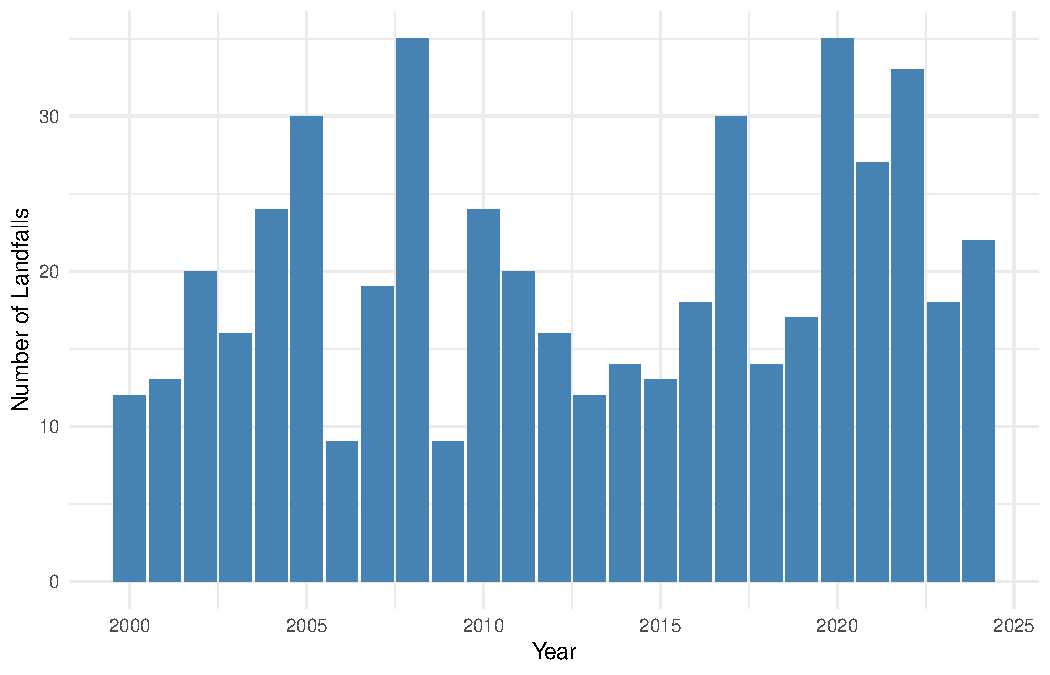
\includegraphics[width=0.49\linewidth,height=1\textheight]{../outputs/eda-hurricane-data/landfalls-per-year} 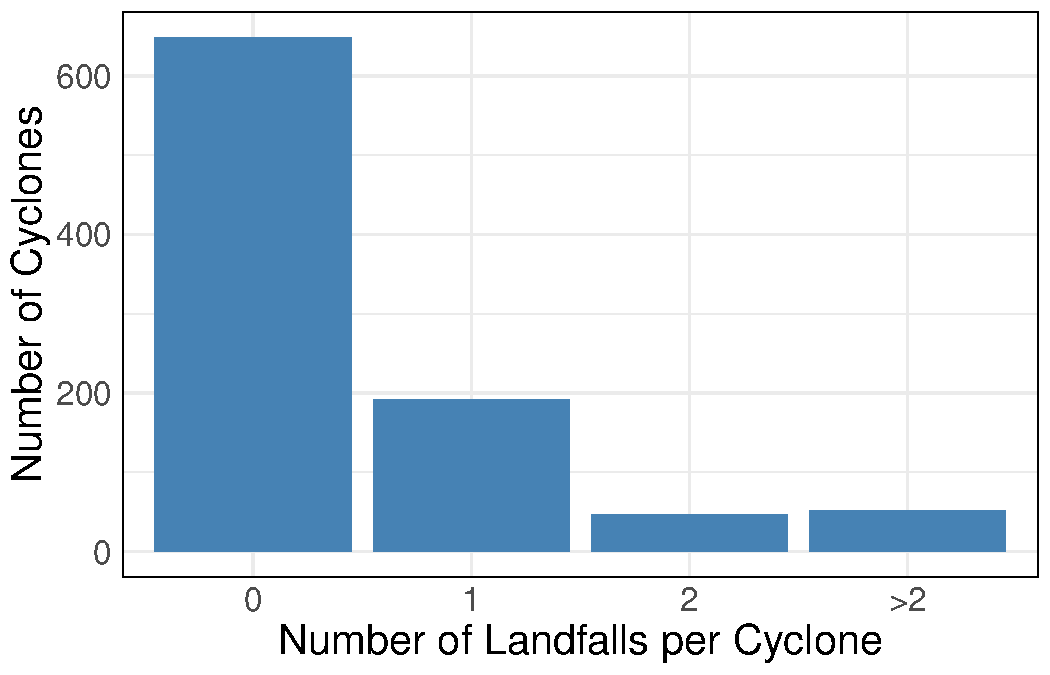
\includegraphics[width=0.49\linewidth,height=1\textheight]{../outputs/eda-hurricane-data/nbr-cyclone-landfalls} 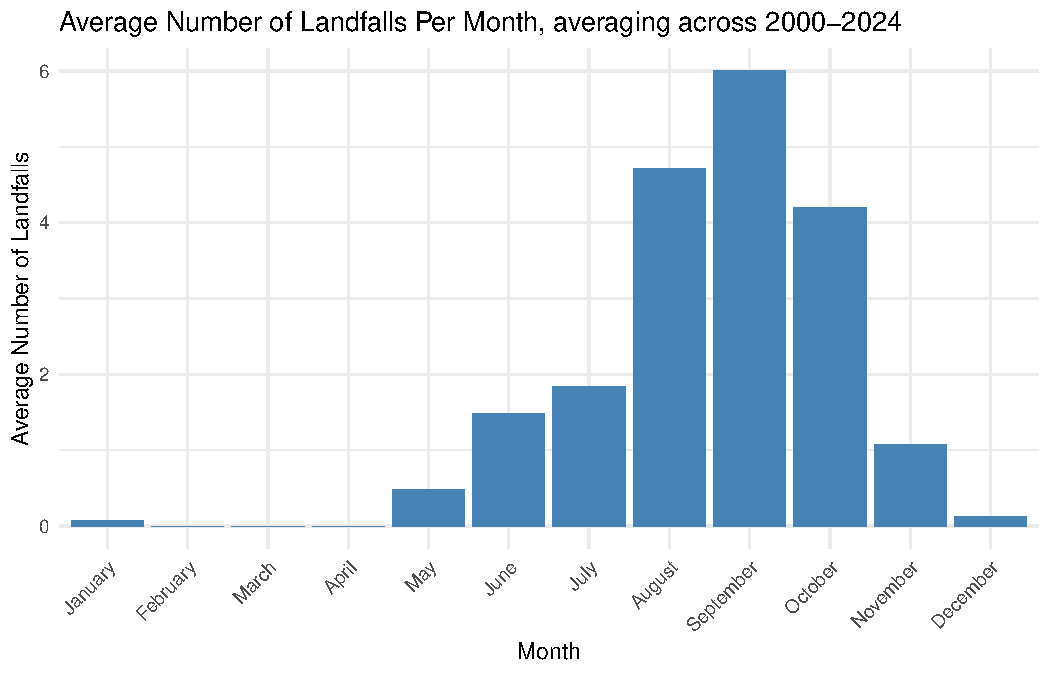
\includegraphics[width=0.49\linewidth,height=1\textheight]{../outputs/eda-hurricane-data/avg-landfalls-per-month} 

}

\caption{(a) Number of cyclone landfalls per year (2000–2024). (b) Number of landfalls per cyclone (2000-2024). (c) Average number of landfalls per month (averaging across 2000-2024).}\label{fig:figs1}
\end{figure}

Figure \ref{fig:figs1} summarises key trends in landfall occurrences over time, including the total number of landfalls per year, the number of landfalls per cyclone, and the average number of landfalls per month. These plots provide insight into both seasonal patterns and the highly variable nature of cyclone landfalls, as well as the typical landfall frequency for each individual tropical cyclone from 2000 to 2024. Annual landfall counts show significant year-to-year fluctuations, reflecting the highly variable nature of cyclone landfalls, whereas the monthly landfall averages show a clear seasonal pattern, with most cyclones making landfall between June and November, consistent with the Atlantic hurricane season (\citeproc{ref-hurricane-season}{Truchelut et al., 2022}). While most tropical cyclones never make landfall, it is important to remember that a single landfall can result in immense destruction of both human life and infrastructure, reinforcing the importance of monitoring these rare yet costly events.

To explore yearly and monthly patterns in cyclone landfalls, we fitted two Bayesian Poisson regression models to our landfall count data, stratified by year and month. These models allowed us to assess both long-term variability and within-year seasonality. The first model (model A) included both a monthly seasonal effect and an annual effect, while the second (model B) focused only on monthly seasonality. Having compared model performance using Leave-One-Out Cross Validation (LOO), we found that both models performed very similarly, although model B provided a slightly better fit to our data, suggesting that there is no consistent long-term trend across the studied 25-year period.

Model B was then used to simulate landfall occurrences in 2025, on a monthly basis, showing an expected peak in landfall activity between August and October.

\begin{figure}

{\centering 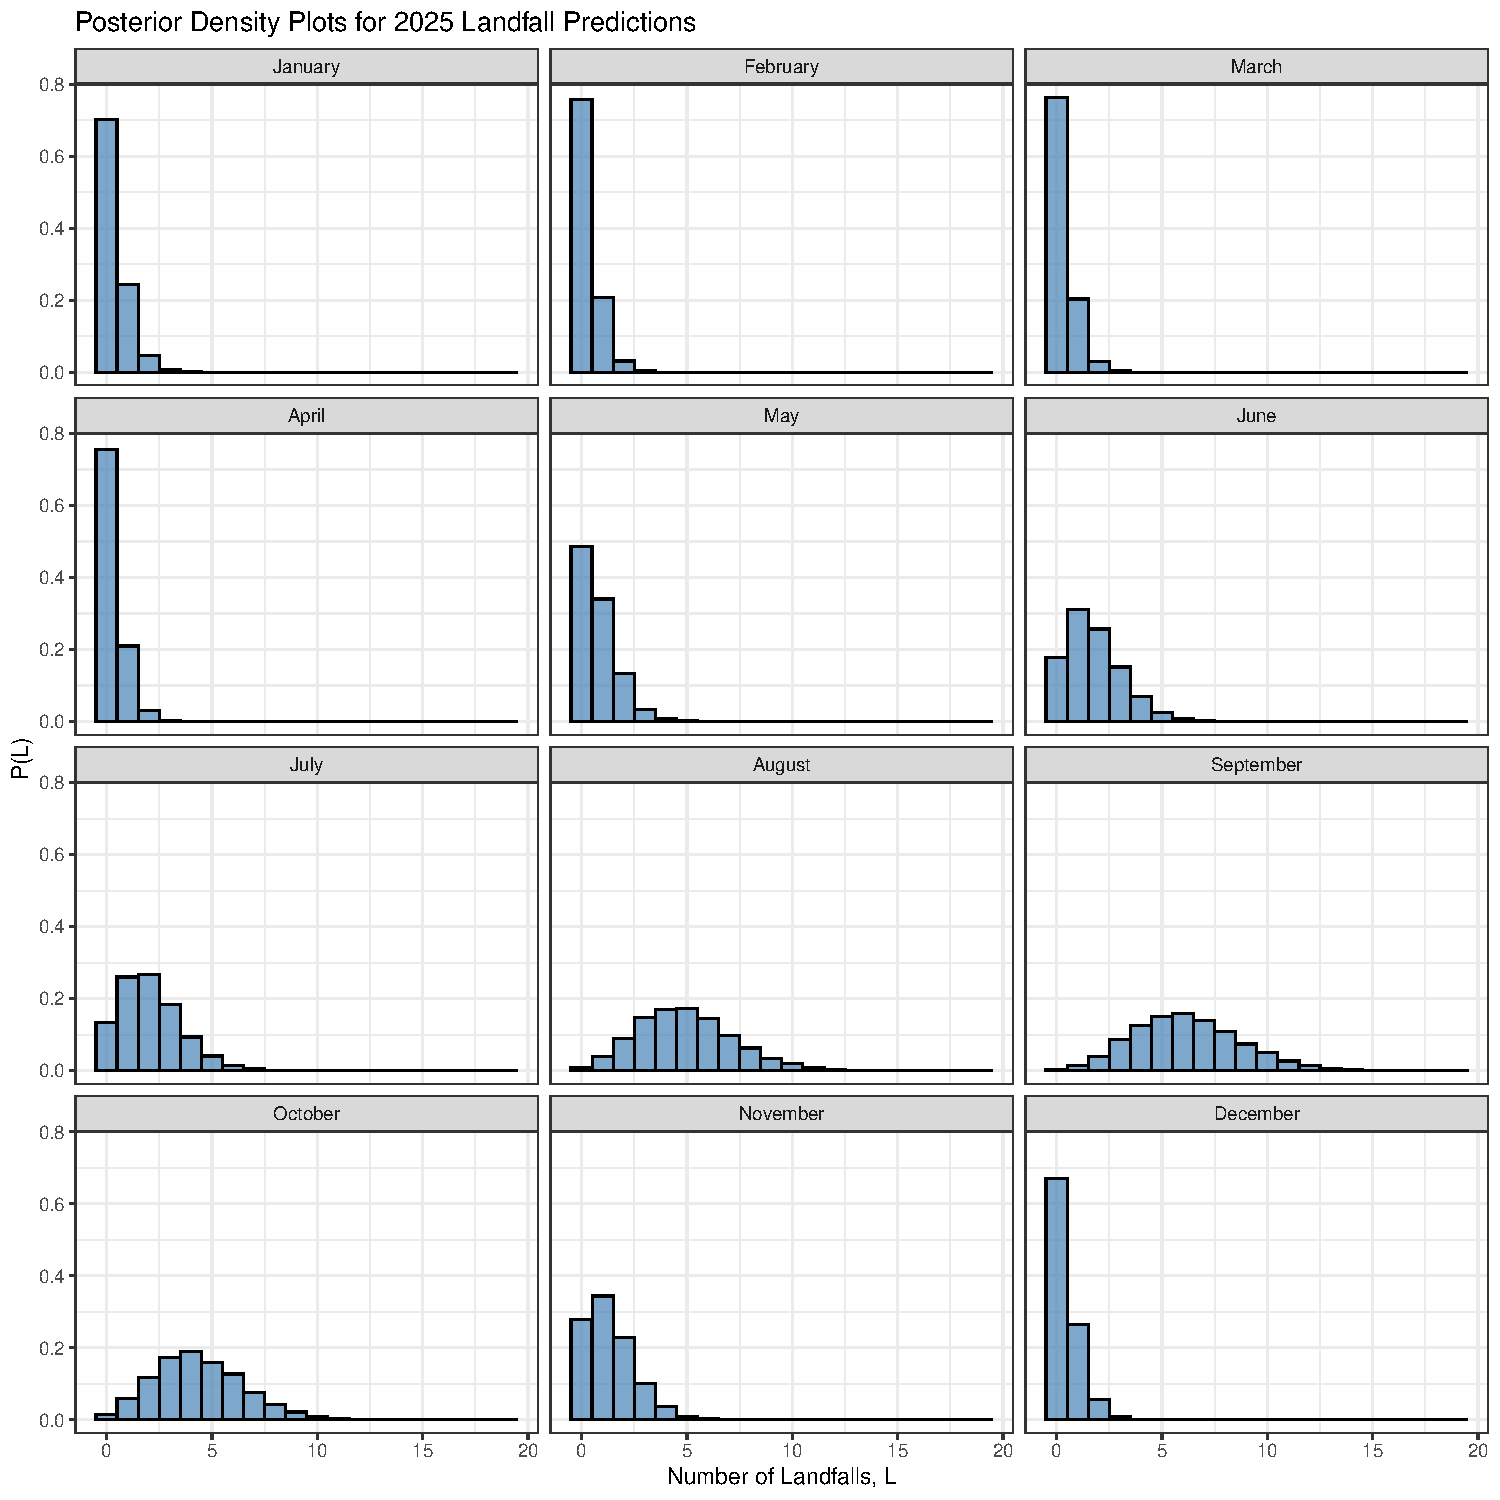
\includegraphics[width=0.82\linewidth]{../outputs/bayesian-analysis-landfall-freq/landfall-monthly-density-plots} 

}

\caption{Estimated probability distribution of cyclone landfalls per month in 2025, based on the seasonal model.}\label{fig:figs2}
\end{figure}

Figure \ref{fig:figs2} shows a clear seasonal pattern in our landfall forecasts, aligning with the typical Atlantic and Pacific hurricane seasons. This figure also emphasises the rarity of landfall occurrences outside of these peak months, with a very low probability of seeing any landfalls at all.

We then took our analysis one step further and examined expected landfall forecasts per month over the next five years (2025-2029).

\begin{figure}

{\centering 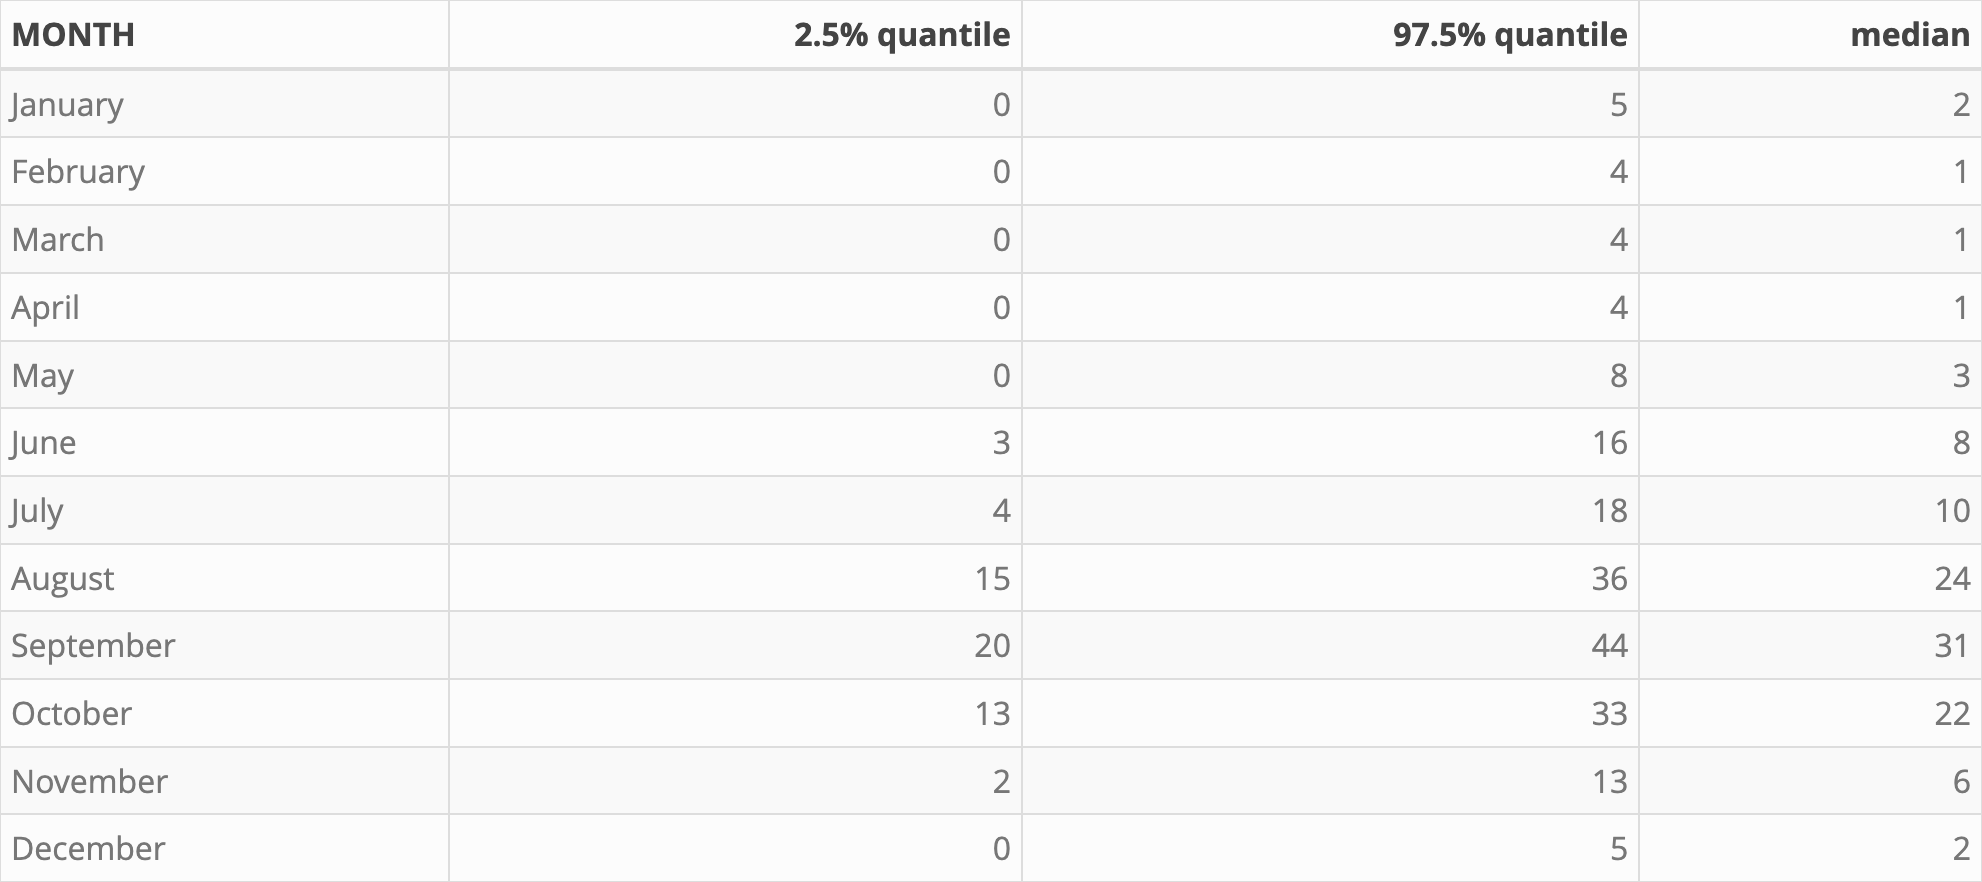
\includegraphics[width=1\linewidth]{../outputs/bayesian-analysis-landfall-freq/simple-landfalls-monthly-forecasts} 

}

\caption{Forecasted number of landfalls per month, 2025-2029, based on the seasonal model.}\label{fig:figs3}
\end{figure}

Figure \ref{fig:figs3} displays the total forecasted number of cyclone landfalls per month from 2025 to 2029, showing the 2.5\% and 97.5\% quantiles and the median value of total landfalls for each month. These values serve as a measure of statistical uncertainty associated with our model. We expect the actual number of total landfalls over this five year period to fall between 2.5\% and 97.5\% quantile values with 95\% certainty.

The forecast predicts the highest number of total landfalls in September, with a median value of 31 landfalls, followed closely by August and October, with median values of 24 and 22 landfalls, respectively. The months of January to April and December are forecasted to experience significantly fewer landfalls, with the median forecast for total landfalls being close to zero in these months.

Our forecasts also highlight the unpredictability of cyclone landfalls, with considerable spread between the 2.5\% quantile and 97.5\% quantile in the June to November months. The wide range of uncertainty in our forecasts for these months underlines the importance of continued research into cyclone activity as to refine and improve model predictions.

\subsection{High-risk countries and territories}\label{high-risk-countries-and-territories}

Before developing our geographical model, we first investigated landfalling cyclone paths from 2000 to 2024. This exploratory analysis plays a crucial role in highlighting cyclone patterns such as intensity, frequency and geographical distribution of landfalls. By visualising cyclone paths and location of landfalls, we can determine which countries and territories are consistently impacted, helping to prioritise areas most in need for our forecasting model.

\begin{figure}

{\centering 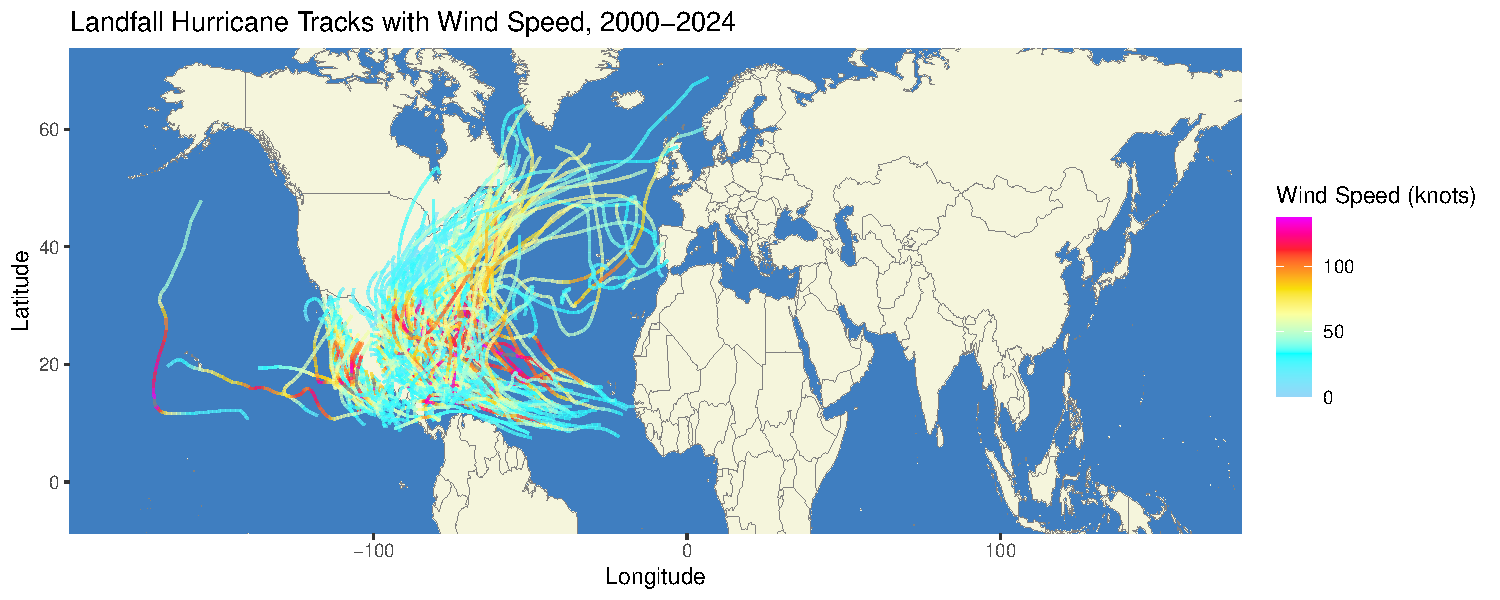
\includegraphics{../outputs/eda-hurricane-data/landfall-map} 

}

\caption{Landfalling cyclone paths in the East Pacific and Atlantic basins, 2000-2024.}\label{fig:figs4}
\end{figure}

Figure \ref{fig:figs4} shows the full path of tropical cyclones that made landfall between 2000 and 2024 across the East Pacific and Atlantic basins. Each path represents an individual cyclone, as well as its wind speed as the cyclone advances. This map highlights how far cyclones can travel before making landfall, emphasising the importance of early detection and consistent monitoring for effective cyclone preparedness.

The erratic nature of cyclone paths, seen by the sudden changes in direction and intensity can leave communities with limited time to evacuate, reinforcing the critical need for raising awareness of regions most vulnerable so governments can enhance response systems, invest in resilient infrastructure and access needed support.

We next took a closer look at landfall locations from 2000 to 2024 in order to identify regions most affected by landfalling cyclones.

\begin{figure}

{\centering 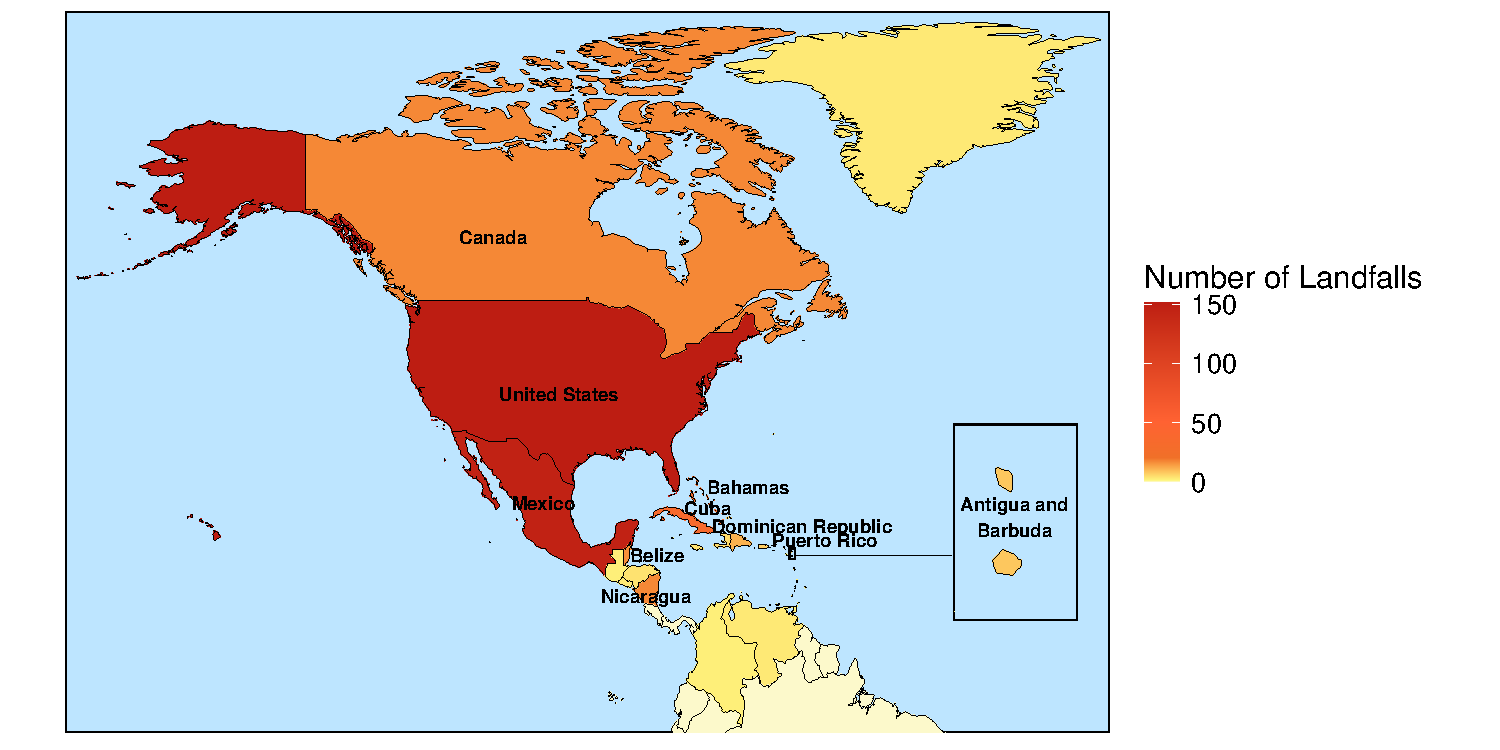
\includegraphics[width=1\linewidth]{../outputs/eda-hurricane-data/landfall-countries} 

}

\caption{Number of tropical cyclone landfalls per country, 2000-2024.}\label{fig:figs5}
\end{figure}

\begin{figure}

{\centering 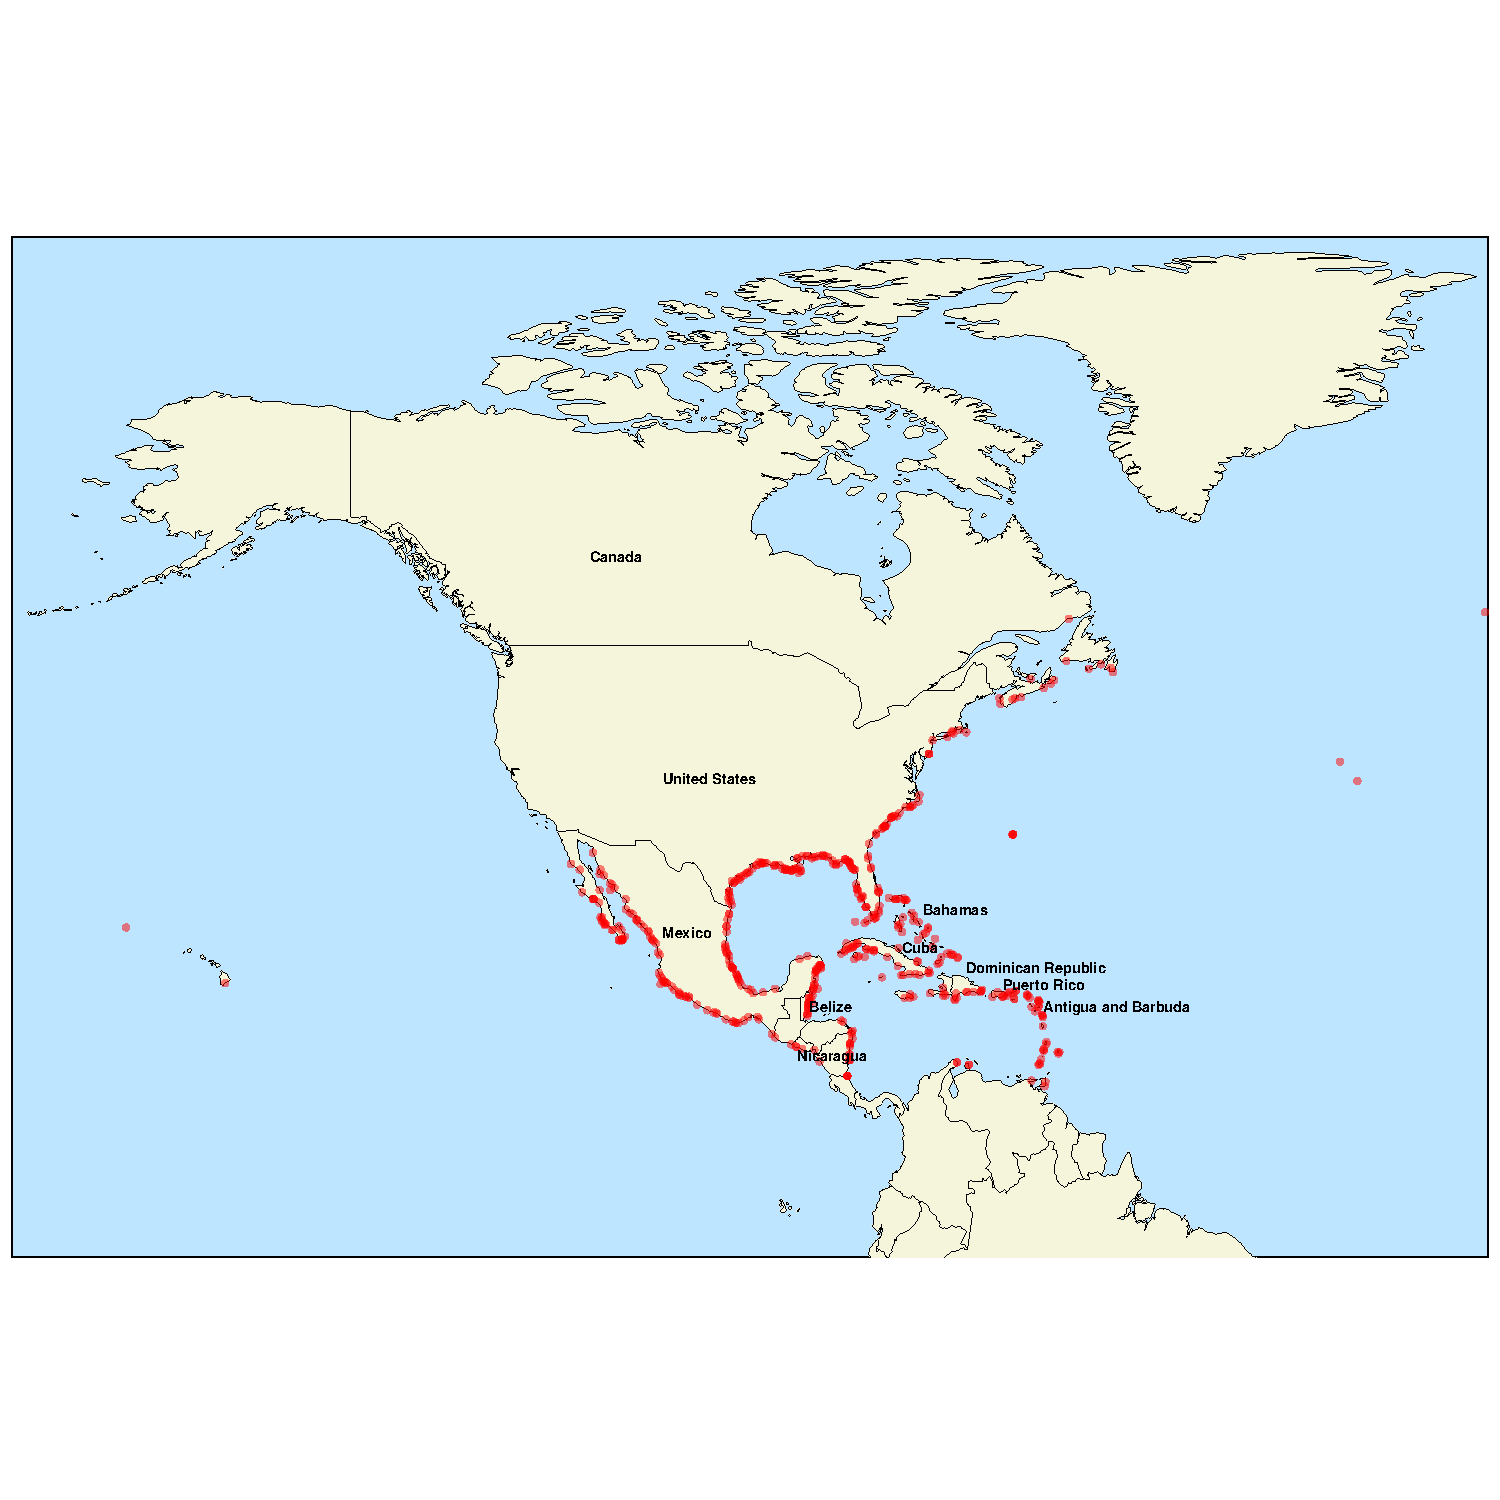
\includegraphics[width=1\linewidth]{../outputs/eda-hurricane-data/landfall-locations} 

}

\caption{Landfall geographical locations, 2000-2024.}\label{fig:figs6}
\end{figure}

Figure \ref{fig:figs5} provides a national-level overview of landfall frequency in the last 25 years, with the United States, Mexico, Nicaragua, the Bahamas, Cuba and Canada standing out as the most impacted by cyclone activity, thus identifying countries with the highest exposure to cyclone landfalls. This is crucial for establishing which governments need the most support.

Figure \ref{fig:figs6}, in contrast, provides a geographical overview of landfall locations since 2000, allowing us to identify which coastal regions are must vulnerable to cyclone activity. We see that the Gulf Coast and East Coast of the United States experience a high number of landfalls, whereas the Pacific coast of the United States hasn't seen any since 2000. On the other hand, both Mexico's East and West coasts have high landfall exposure. This map is particularly important for local disaster preparedness, showing which areas are most susceptible to damages caused by cyclone landfalls.

To explore geographical patterns in cyclone landfalls, we fitted a Bayesian Poisson regression model to our landfall count data, now stratified by year and location. This model (model C) allowed us to assess country and territory-level vulnerability related to cyclone landfalls. Model C ignores yearly time trends based on the results of our previous time-based models (where we saw a better performance from our model without a year effect). Instead, model C incorporates country and territory-level effects for the top ten countries with the most landfalls since 2000: the United States of America, Mexico, Cuba, the Bahamas, Nicaragua, Canada, Belize, Dominican Republic, Antigua and Barbuda and Puerto Rico, as seen in Figure \ref{fig:figs5}.

We then used model C to simulate landfall occurrences in 2025, for each of the countries and territories in our top ten list. Figure \ref{fig:figs7} clearly isolated the United States of America and Mexico as the most vulnerable regions in 2025, even amongst the top ten landfall-exposed countries. This figure reinforces the rarity of landfall occurrences outside of these two countries, with other countries having a very low probability of seeing any landfalls.

\newpage

\begin{figure}

{\centering 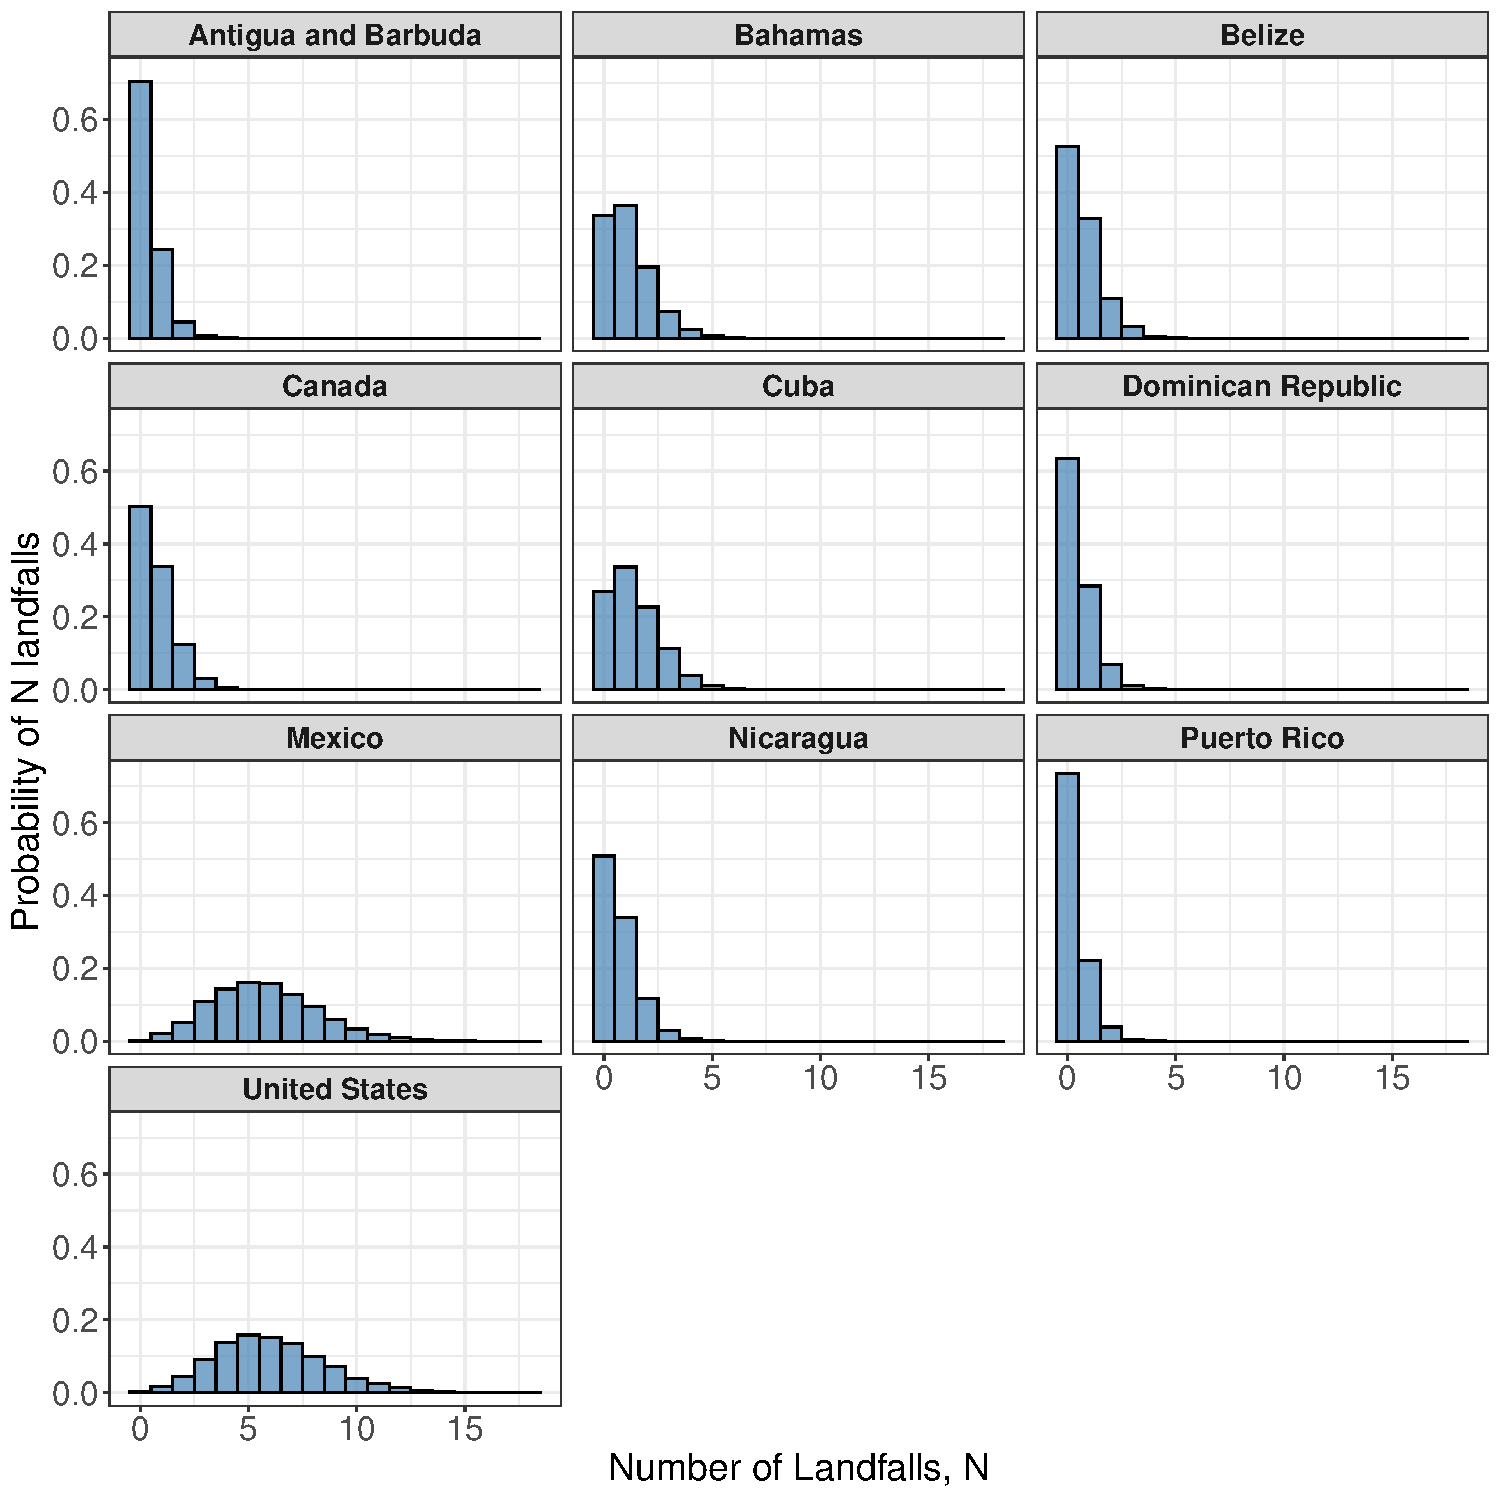
\includegraphics[width=0.82\linewidth]{../outputs/bayesian-analysis-country-freq/landfall-per-country-density-plots} 

}

\caption{Estimated probability distribution of cyclone landfalls per country and territory in 2025.}\label{fig:figs7}
\end{figure}

We then took our analysis one step further and examined expected landfall forecasts for each of our top ten countries and territories over the next five years (2025-2029).

\begin{figure}

{\centering 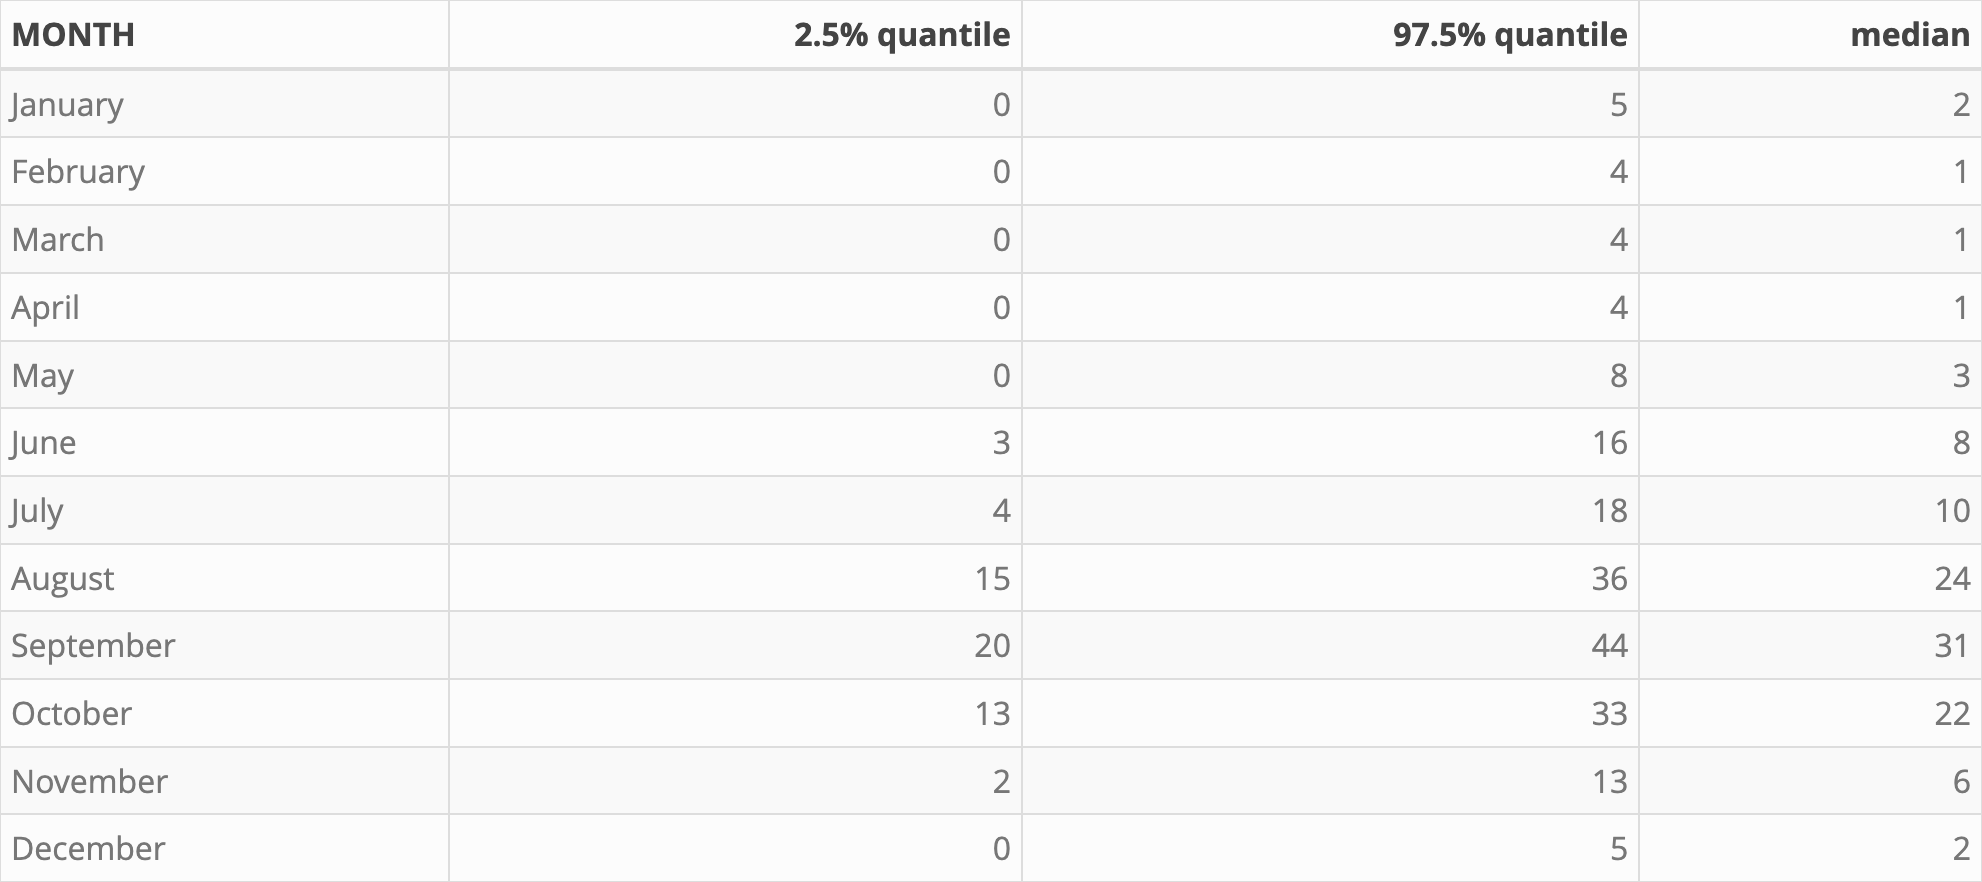
\includegraphics[width=1\linewidth]{../outputs/bayesian-analysis-country-freq/simple-landfalls-per-country-forecasts} 

}

\caption{Forecasted number of landfalls per country and territory, 2025-2029.}\label{fig:figs8}
\end{figure}

Figure \ref{fig:figs8} displays the total forecasted number of cyclone landfalls per country and territory from 2025 to 2029, showing the 2.5\% and 97.5\% quantiles and the median value of total landfalls for each month.

The forecast predicts the highest number of total landfalls in the United States of America, followed closely by Mexico , with median values of 30 and 29 landfalls, respectively. Puerto Rico, the Dominican Republic and Antigua and Barbuda have the lowest forecasted landfalls, with a median value of total landfalls over the next 5 years close to zero, despite being in the top ten most exposed countries and territories.

Our forecasts once again highlight the unpredictability of cyclone landfalls, with considerable spread between the 2.5\% and 97.5\% quantiles for some of our countries and territories such as the United States of America, Mexico, the Bahamas and Cuba. The wide range of uncertainty in our forecasts for these countries once again underlines the importance of continued research into cyclone activity as to refine and improve model predictions.

\section{Recommendations}\label{recommendations}

Based on our analysis of historical landfall patterns and probabilistic forecasts, we recommend the following actions to reinforce cyclone preparedness and resource allocation:

\begin{itemize}
\tightlist
\item
  Allocate emergency supplies and necessary resources ahead of the peak season (June to November) with response units in place and ready to act, especially in August to October, when the probability of landfalls reaches a peak.
\item
  Prioritise the United States of America and Mexico, followed by the Bahamas and Cuba, for storing medical kits, food, water, and to put in place temporary shelters.
\item
  Support local authorities in vulnerable areas through evacuation drills and strengthening infrastructure (especially hospitals, schools, and emergency shelters).
\end{itemize}

By aligning these targets with the seasonal and geographic insights from our models, organisations can reduce disaster response times, minimise casualties, and accelerate recovery.

\section{Limitations of models and data biases}\label{limitations-of-models-and-data-biases}

While our Bayesian Poisson regression models provide valuable insights, several limitations should be considered:

\begin{itemize}
\tightlist
\item
  Landfall coordinates which fell over water were mapped to the nearest country, introducing geographical uncertainty.
\item
  Our models treated all landfalls equally, without distinguishing storm intensity or amount of damage caused.
\item
  The data used in our model was sparse, and the resulting choice to ignore yearly time trends in cyclone behaviour over 2000--2024, may lead to inaccuracies due to accelerating climate change.
\item
  Wide credible intervals in our five‑year forecasts reflect both variability and uncertainty in our forecasts.
\item
  Our models do not account for population density, infrastructure quality, or socioeconomic resilience, which influence actual humanitarian need. While countries like the United States may experience the highest number of landfalls, their relatively stronger economic resilience allows for stronger infrastructure and faster recovery. In contrast, economically weaker countries in the region may face catastrophic consequences from even a single cyclone landfall. These regions might rely more heavily on humanitarian aid to reduce the impact of cyclone landfalls on vulnerable populations and infrastructure.
\end{itemize}

\section{Conclusion}\label{conclusion}

This report demonstrates a clear seasonal cycle in tropical cyclone landfalls, with most occurring between June and November. Our results indicate that there is no significant trend in annual landfall counts from 2000 to 2024. Moreover, our forecasts identify the United States and Mexico as the highest‑risk countries over the next five years, with a substantial probability of multiple landfalls in each hurricane season.

Through our use of Bayesian models, we hope to provide actionable insights to help humanitarian agencies and governments optimise cyclone preparedness and resource allocation. Despite some uncertainties and data limitations, these findings offer a foundation for region-specific disaster risk reduction efforts.

\section{References}\label{references}

\phantomsection\label{refs}
\begin{CSLReferences}{0}{1}
\bibitem[\citeproctext]{ref-landfall-damages}
Baradaranshoraka, M., Pinelli, J.-P., Gurley, K., Peng, X. \& Zhao, M. (2017) Hurricane wind versus storm surge damage in the context of a risk prediction model. \emph{Journal of Structural Engineering}. 143 (9), 04017103. doi:\href{https://doi.org/10.1061/(ASCE)ST.1943-541X.0001824}{10.1061/(ASCE)ST.1943-541X.0001824}.

\bibitem[\citeproctext]{ref-Elsner}
Elsner, J.B., Bossak, B.H. \& Niu, X.-F. (2001) Secular changes to the ENSO-u.s. Hurricane relationship. \emph{Geophysical Research Letters}. 28 (21), 4123--4126. doi:\url{https://doi.org/10.1029/2001GL013669}.

\bibitem[\citeproctext]{ref-casualties}
Li, K. \& Li, G. (2013) {Risk assessment on storm surges in the coastal area of Guangdong Province}. \emph{Natural Hazards: Journal of the International Society for the Prevention and Mitigation of Natural Hazards}. 68 (2), 1129--1139. doi:\href{https://doi.org/10.1007/s11069-013-0682-2}{10.1007/s11069-013-0682-2}.

\bibitem[\citeproctext]{ref-eastern-pacific}
Ocegueda Sanchez, J.A., Chavas, D.R. \& Jones, J.J. (2025) Interannual variability of tropical cyclone landfalls in the eastern north pacific: Environmental drivers and implications. \emph{Geophysical Research Letters}. 52 (8), e2024GL113807. doi:\url{https://doi.org/10.1029/2024GL113807}.

\bibitem[\citeproctext]{ref-hurricane-season}
Truchelut, R.E., Klotzbach, P.J., Staehling, E.M., Wood, K.M., Halperin, D.J., Schreck, C.J. \& Blake, E.S. (2022) Earlier onset of {North} {Atlantic} hurricane season with warming oceans. \emph{Nature Communications}. 13 (1), 4646. doi:\href{https://doi.org/10.1038/s41467-022-31821-3}{10.1038/s41467-022-31821-3}.

\end{CSLReferences}

\newpage

\section{Appendix - Technical description of analysis and data processing}\label{appendix---technical-description-of-analysis-and-data-processing}

\subsection{Data processing}\label{data-processing}

Both the Atlantic and Northeast and North Central Pacific hurricane databases (HURDAT2) contain cyclone information recorded at six hour intervals as well as when a cyclone changes status unexpectedly. The information contained in each row of these databases includes:

\begin{itemize}
\tightlist
\item
  storm ID (contains Basin, year, and cyclone number for that year);
\item
  name, if available;
\item
  number of recorded track data for each cyclone;
\item
  date;
\item
  time;
\item
  record identifier (identifies landfalls or indicates a reason for the inclusion of the record outside of the regular six hour intervals);
\item
  cyclone position (measured in latitude and longitude);
\item
  system status;
\item
  maximum sustained wind (in knots);
\item
  minimum pressure (in millibars);
\item
  radius of maximum wind (in nautical miles).
\end{itemize}

For the purpose of this report, the two databases were combined and the following features were extracted from cyclones in 2000 to 2024:

\begin{itemize}
\tightlist
\item
  storm ID;
\item
  name, if available;
\item
  day;
\item
  month;
\item
  year;
\item
  time;
\item
  record identifier;
\item
  cyclone position (measured in latitude and longitude, converted to positive and negative decimals);
\item
  system status;
\item
  maximum sustained wind (in knots, converted to integers);
\item
  minimum pressure (in millibars, converted to integers).
\end{itemize}

This data set was then used to identify all landfall events in the studied period, using the record identifier ``L''. We then matched our landfall data to countries and territories in the North American continent, using vector maps of country and territory boundaries. If the latitude and longitude coordinates of a landfall did not fall within a country or territory boundary, we matched it to the closest country or territory boundary point. This finalised landfall data set, containing geographical information was then used for all the models in this study.

\subsubsection{Monthly and yearly landfall frequency (Models A and B)}\label{monthly-and-yearly-landfall-frequency-models-a-and-b}

For both seasonal models A and B, landfalls were grouped by month and year, from 2000 to 2024.
We then counted the number of landfalls in each group and matched this to all month and year combinations, in order to count which groups (month/year combinations) had zero landfalls.

We gave each month a numerical ID number, ranging from 1 to 12 (January to December) and we included our prediction data for 2025 to 2029, with unknown counts, at the end of our seasonal landfall frequency data set.

Finally, years were standardised to the range {[}-1,1{]} using the following formula:

\[\text{standardised year} = \frac{\text{year} - 2000}{2029 - 2000}\].

\subsubsection{Geographical landfall frequency (Model C)}\label{geographical-landfall-frequency-model-c}

The top 10 most exposed countries and territories were identified based on total number of landfalls in the studied period.

We then filtered our landfalls data set to only include these 10 countries and territories, and grouped landfalls by year and country or territory (location), from 2000 to 2024.
We then counted the number of landfalls in each group and matched this to all location and year combinations, in order to count keep track of the groups with zero landfalls.

Similarly to our previous frequency data set, we gave each location a numerical ID number, ranging from 1 to 10 and we included our prediction data for 2025 to 2029, with unknown counts, at the end of our data set.

Finally, we encoded the location information in our geographical count data set using a one-hot design matrix, where each row matches a year-location combination and each column represents a location and contains a 1 if the row matches the location, or a 0 otherwise.

\subsection{Model A: Monthly seasonal model with yearly effect}\label{model-a-monthly-seasonal-model-with-yearly-effect}

Our first model represents a Bayesian Poisson Regression model, with a monthly seasonality effect, and a non-linear yearly effect (modeled using a Gaussian Process). This model was fitted using Markov Chain Monte Carlo (MCMC) methods.

Mathematically, our model is denoted:

\begin{align*}
&Y_{i} \sim \text{Poisson}(\lambda_{i})\\
&\text{log } \lambda_{i} =  \beta_{m(i)} + f(T(i))\\
&\beta \sim \text{N}( 0, \frac{M}{M-1}( I - \frac{1}{M} \mathbf{1}\mathbf{1}^T) \cdot \sigma_{\beta}^2), \text{  (sum-to-zero constraint)}\\
& f \sim \text{HSGP}(\alpha, \rho)\\
&\sigma_{\beta} \sim \text{Half-Cauchy}(0,1)\\
&\alpha \sim \text{Half-Cauchy}(0,1) \\
&\rho \sim \text{Inv-Gamma}(5,1)
\end{align*}

where

\begin{itemize}
\tightlist
\item
  \(i\) indexes observations, \(i=1,...,300\);
\item
  \(M\) is the number of months, \(M = 12\);
\item
  \(Y_{i}\) is the observed count of landfalls for observation \(i\);
\item
  \(m(i)\) is a map from \(i\) (the observations) to the corresponding month ID (integers between \(1\) and \(12\));
\item
  \(T(i)\) is a map from \(i\) (the observations) to the corresponding standardised year;
\item
  \(\beta \in \mathbb{R}^{12}\) is the monthly seasonal effect, where \(\beta_1\) is the effect for month 1 (January), \(\beta_2\) is the effect for month 2 (February) and so on;
\item
  \(f\) is given a zero-mean HSGP prior with squared exponential kernel with GP variance \(\alpha\) and length scale \(\rho\).\\
\item
  \(\sigma_{\beta}\) scales the variance of \(\beta\) to implement non-centered parameterisation on top of the sum-to-zero constraint, where both constraints are methods implemented to improve parameter identifiability, sampling efficiency and convergence of our model parameters;
\item
  \(\lambda_{i}\) is the expected number of landfalls per month and year
\end{itemize}

We ran our MCMC algorithm using 3 parallel Markov chains, 4000 iterations, discarding the first 500 as ``warm-up'' iterations. We verified model convergence by investigating key model parameter convergence diagnostics, as well as checking trace plots for our worst performing parameter and looking at pairwise posterior geometries (thus allowing us to verify that all our parameters are identifiable).

\begin{figure}

{\centering 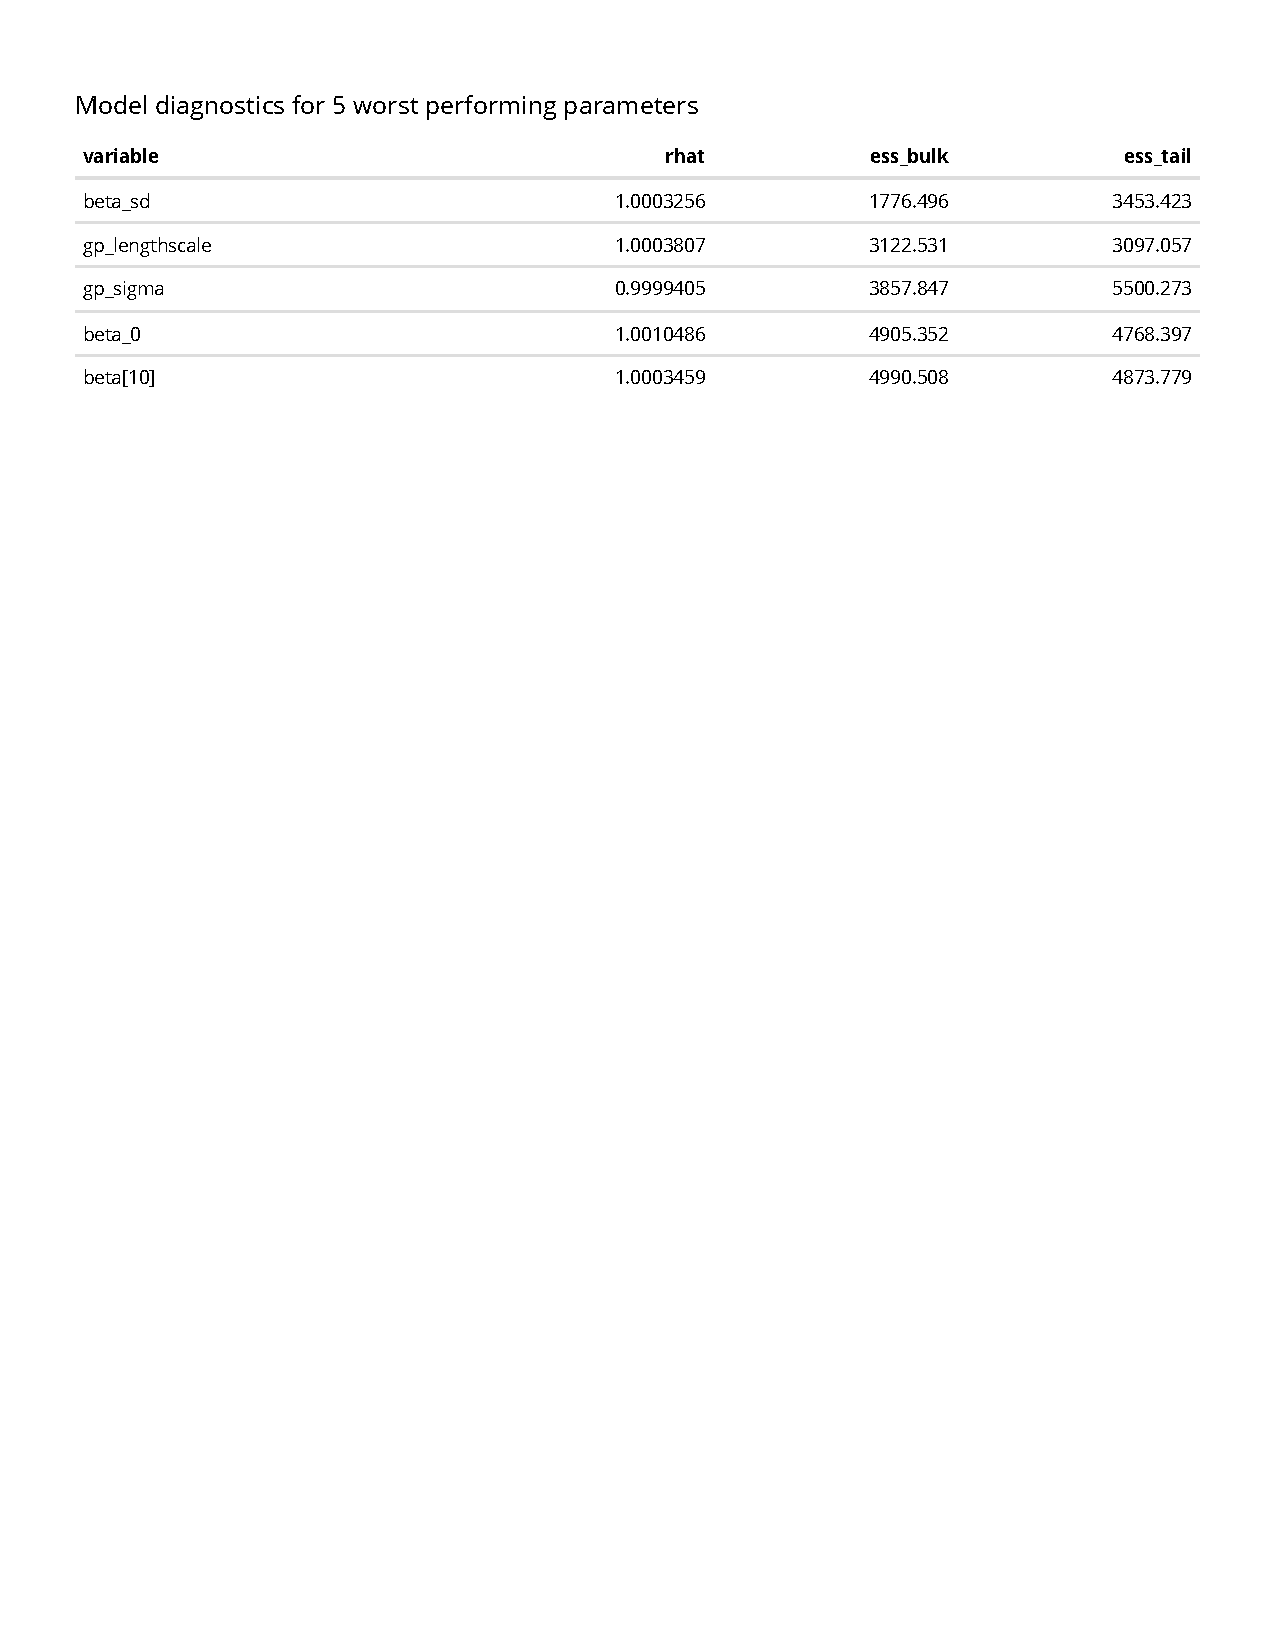
\includegraphics[width=1\linewidth]{../outputs/bayesian-analysis-landfall-freq/model-HSGP/HSGP-model-diagnostics} 

}

\caption{Model convergence diagnostics for our 5 worst performing parameters.}\label{fig:figs9}
\end{figure}

Figure \ref{fig:figs9} displays 3 statistical efficiency and convergence measures for our worst performing parameters (in terms of the ``ess\_bulk'' measure, where a lower ``ess\_bulk'' value represents lower efficiency). In general, for convergence, we expect an ``rhat'' value close to 1, and for efficiency we expect ``ess\_bulk'' and ``ess\_tail'' values greater than 1500 (500 for each parallel chain). As we can see, all ``rhat'' convergence diagnostic values are less than 1.01, which suggests good mixing and convergence. Moreover both ``ess\_tail'' and ``ess\_bulk'' suggest good sampling efficiency (as they are greater than 500 per Markov chain, a common baseline for efficiency in Bayesian MCMC models).

We then checked model fit by performing a posterior predictive check (we simulate data from our model's posterior distribution and compare these to the actual observed data to see if our model explains the data well). To verify model fit, we calculated the probability that an observed data point lies in the 95\% credible interval of the corresponding posterior distribution.

\begin{figure}

{\centering 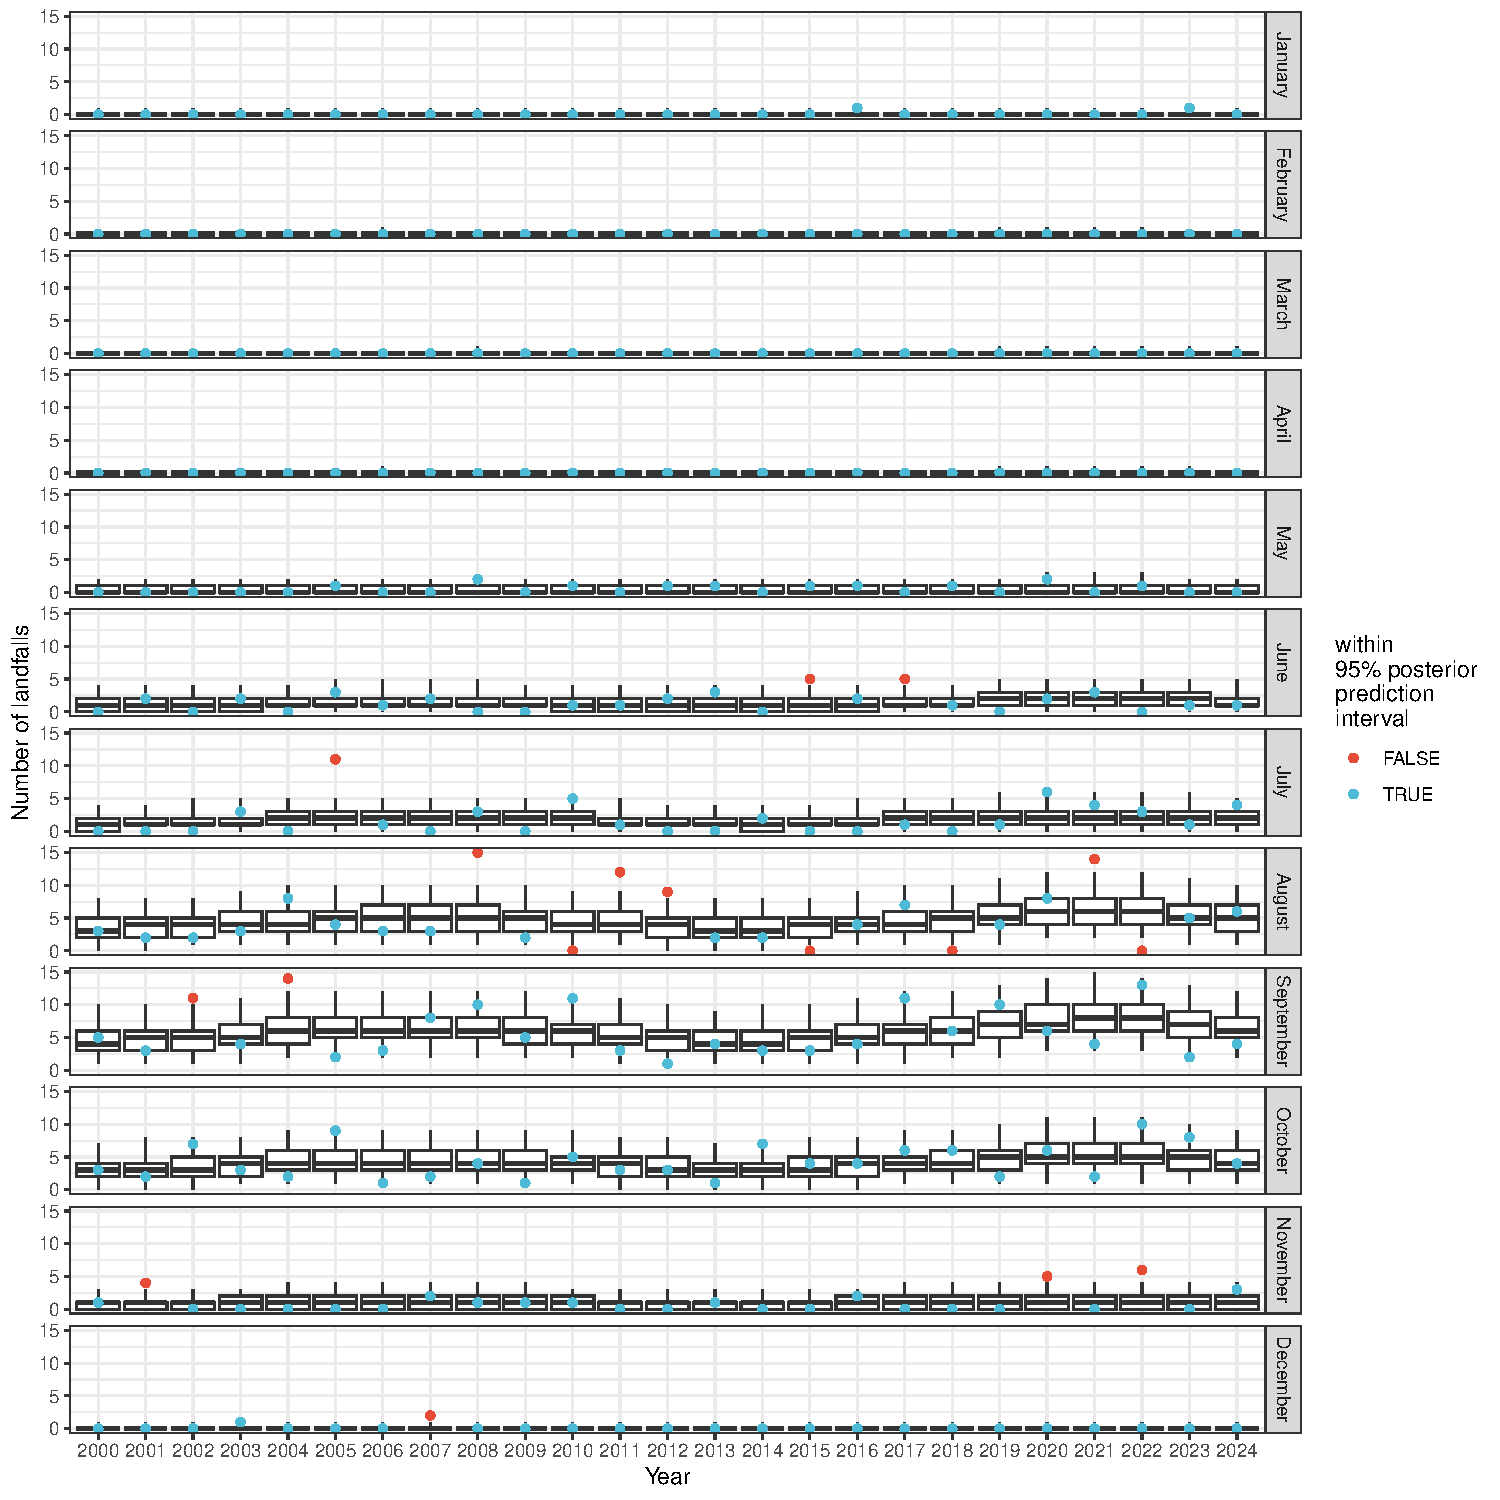
\includegraphics[width=1\linewidth]{../outputs/bayesian-analysis-landfall-freq/model-HSGP/HSGP-post-pred-checks} 

}

\caption{95\% posterior credible intervals and observed data for each month and year, 2000-2024.}\label{fig:figs10}
\end{figure}

We found that 95.7\% of our observed landfall counts fell within our model's posterior predictive intervals, suggesting a good model fit. This can be seen in Figure \ref{fig:figs10}.

\newpage

\subsection{Model B: Monthly seasonal model without yearly effect}\label{model-b-monthly-seasonal-model-without-yearly-effect}

Our second model represents a Bayesian Poisson Regression model, with a monthly seasonality effect. This model was also fitted using Markov Chain Monte Carlo (MCMC) methods.

Mathematically, our model is denoted:

\begin{align*}
&Y_{i} \sim \text{Poisson}(\lambda_{i})\\
&\text{log } \lambda_{i} =  \beta_{m(i)}\\
&\beta \sim \text{MVN}( 0, \frac{M}{M-1}( I - \frac{1}{M} \mathbf{1}\mathbf{1}^T) \cdot \sigma_{\beta}^2), \text{  (sum-to-zero constraint)}\\
&\sigma_{\beta} \sim \text{Half-Cauchy}(0,1)\\
\end{align*}

where

\begin{itemize}
\tightlist
\item
  \(i\) indexes observations, \(i=1,...,300\);
\item
  \(M\) is the number of months, \(M = 12\);
\item
  \(Y_{i}\) is the observed count of landfalls for observation \(i\);
\item
  \(m(i)\) is a map from \(i\) (the observations) to the corresponding month ID (integers between \(1\) and \(12\));
\item
  \(\beta \in \mathbb{R}^{12}\) is the monthly seasonal effect, where \(\beta_1\) is the effect for month 1 (January), \(\beta_2\) is the effect for month 2 (February) and so on;
\item
  \(\sigma_{\beta}\) scales the variance of \(\beta\) to implement non-centered parameterisation on top of the sum-to-zero constraint, where both constraints were implemented to improve parameter identifiability, sampling efficiency and convergence of our model parameters;
\item
  \(\lambda_{i}\) is the expected number of landfalls per month and year
\end{itemize}

Similarly to model A, we ran our MCMC algorithm using 3 parallel Markov chains, 4000 iterations, discarding the first 500 as ``warm-up'' iterations. We verified model convergence by investigating key model parameter convergence diagnostics, as well as checking the trace plot for our worst performing parameter and looking at pairwise posterior geometries (allowing us to verify that all our parameters are identifiable).

\begin{figure}

{\centering 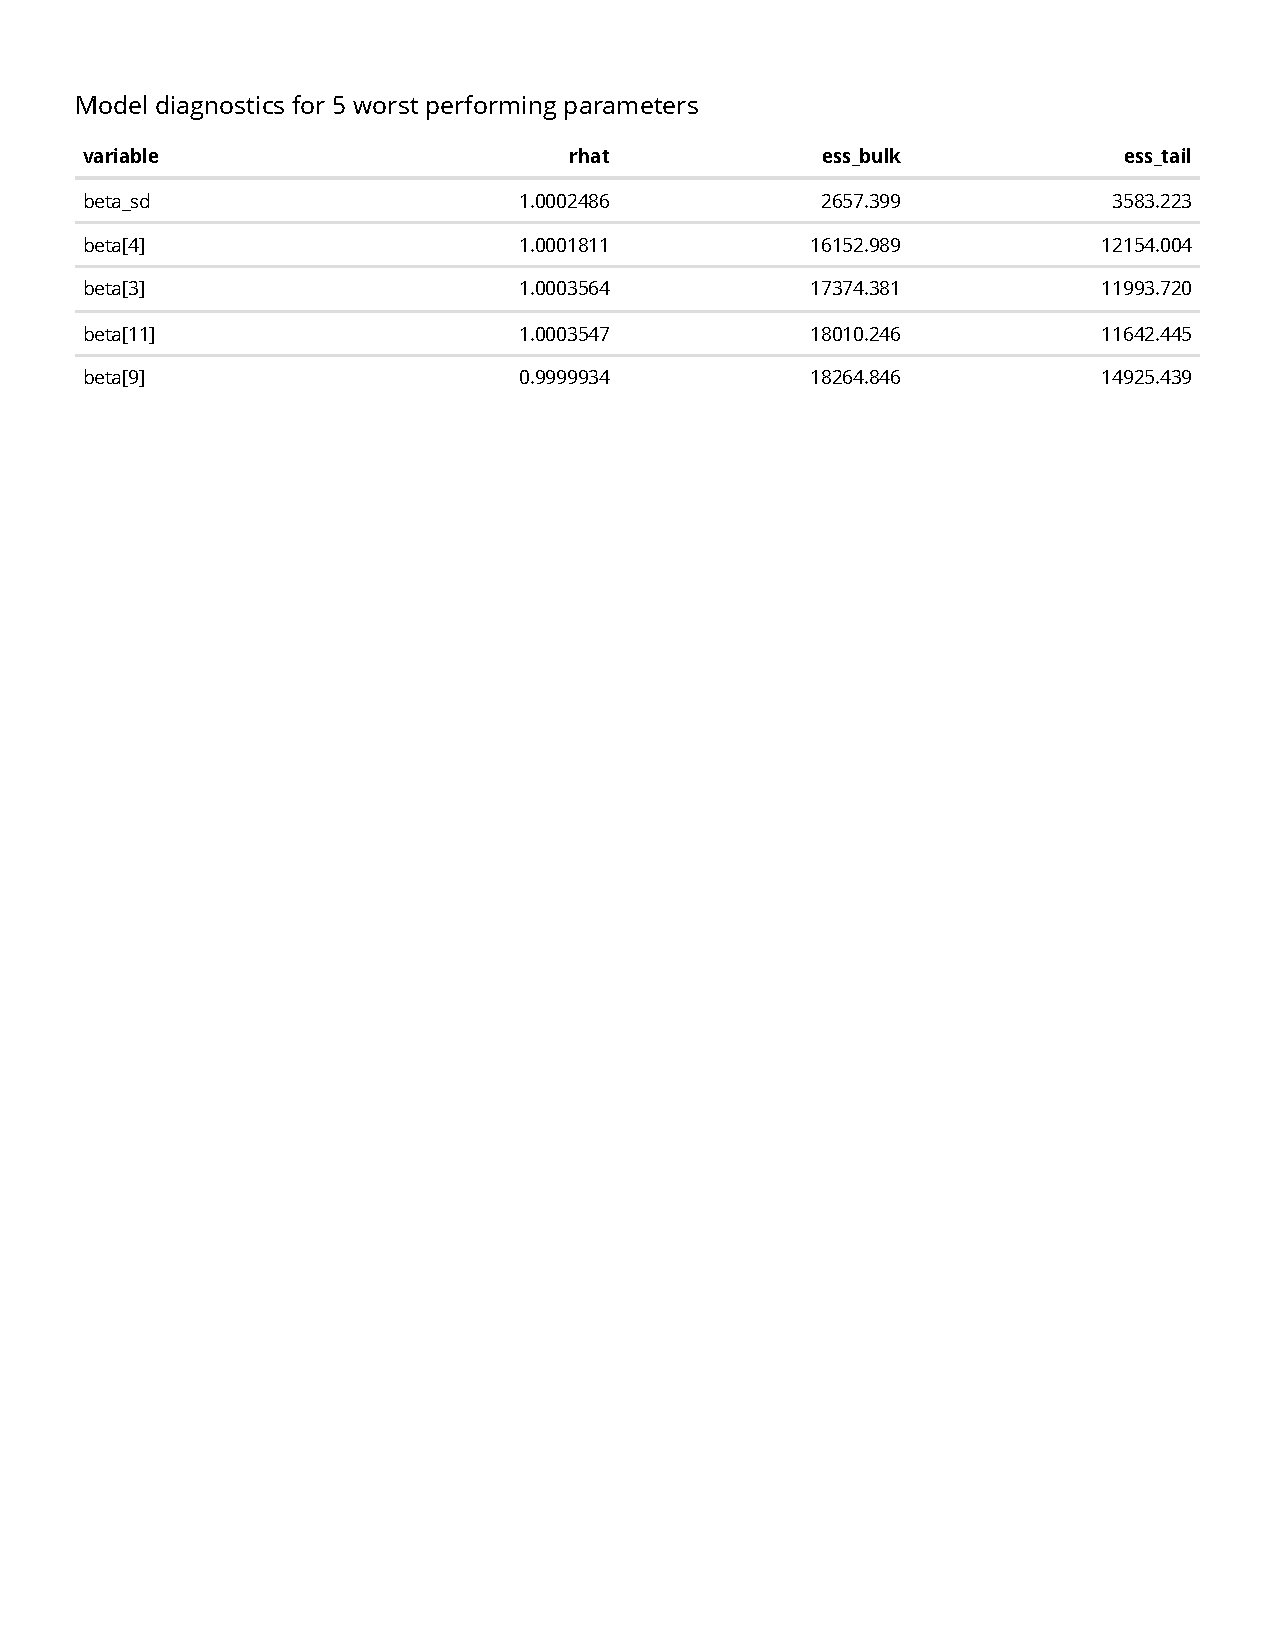
\includegraphics[width=1\linewidth]{../outputs/bayesian-analysis-landfall-freq/model-no-year-effect/no-year-model-diagnostics} 

}

\caption{Model convergence diagnostics for our 5 worst performing parameters.}\label{fig:figs11}
\end{figure}

Figure \ref{fig:figs11} displays the 3 statistical efficiency and convergence measures for our worst performing parameters (in terms of the ``ess\_bulk'' measure). As we can see, all ``rhat'' convergence diagnostic values are less than 1.01, which suggests good mixing and convergence. Moreover both ``ess\_tail'' and ``ess\_bulk'' suggest good sampling efficiency (as they are greater than 500 per Markov chain).

We then checked model fit by performing a posterior predictive check, similarly to Model A.

\begin{figure}

{\centering 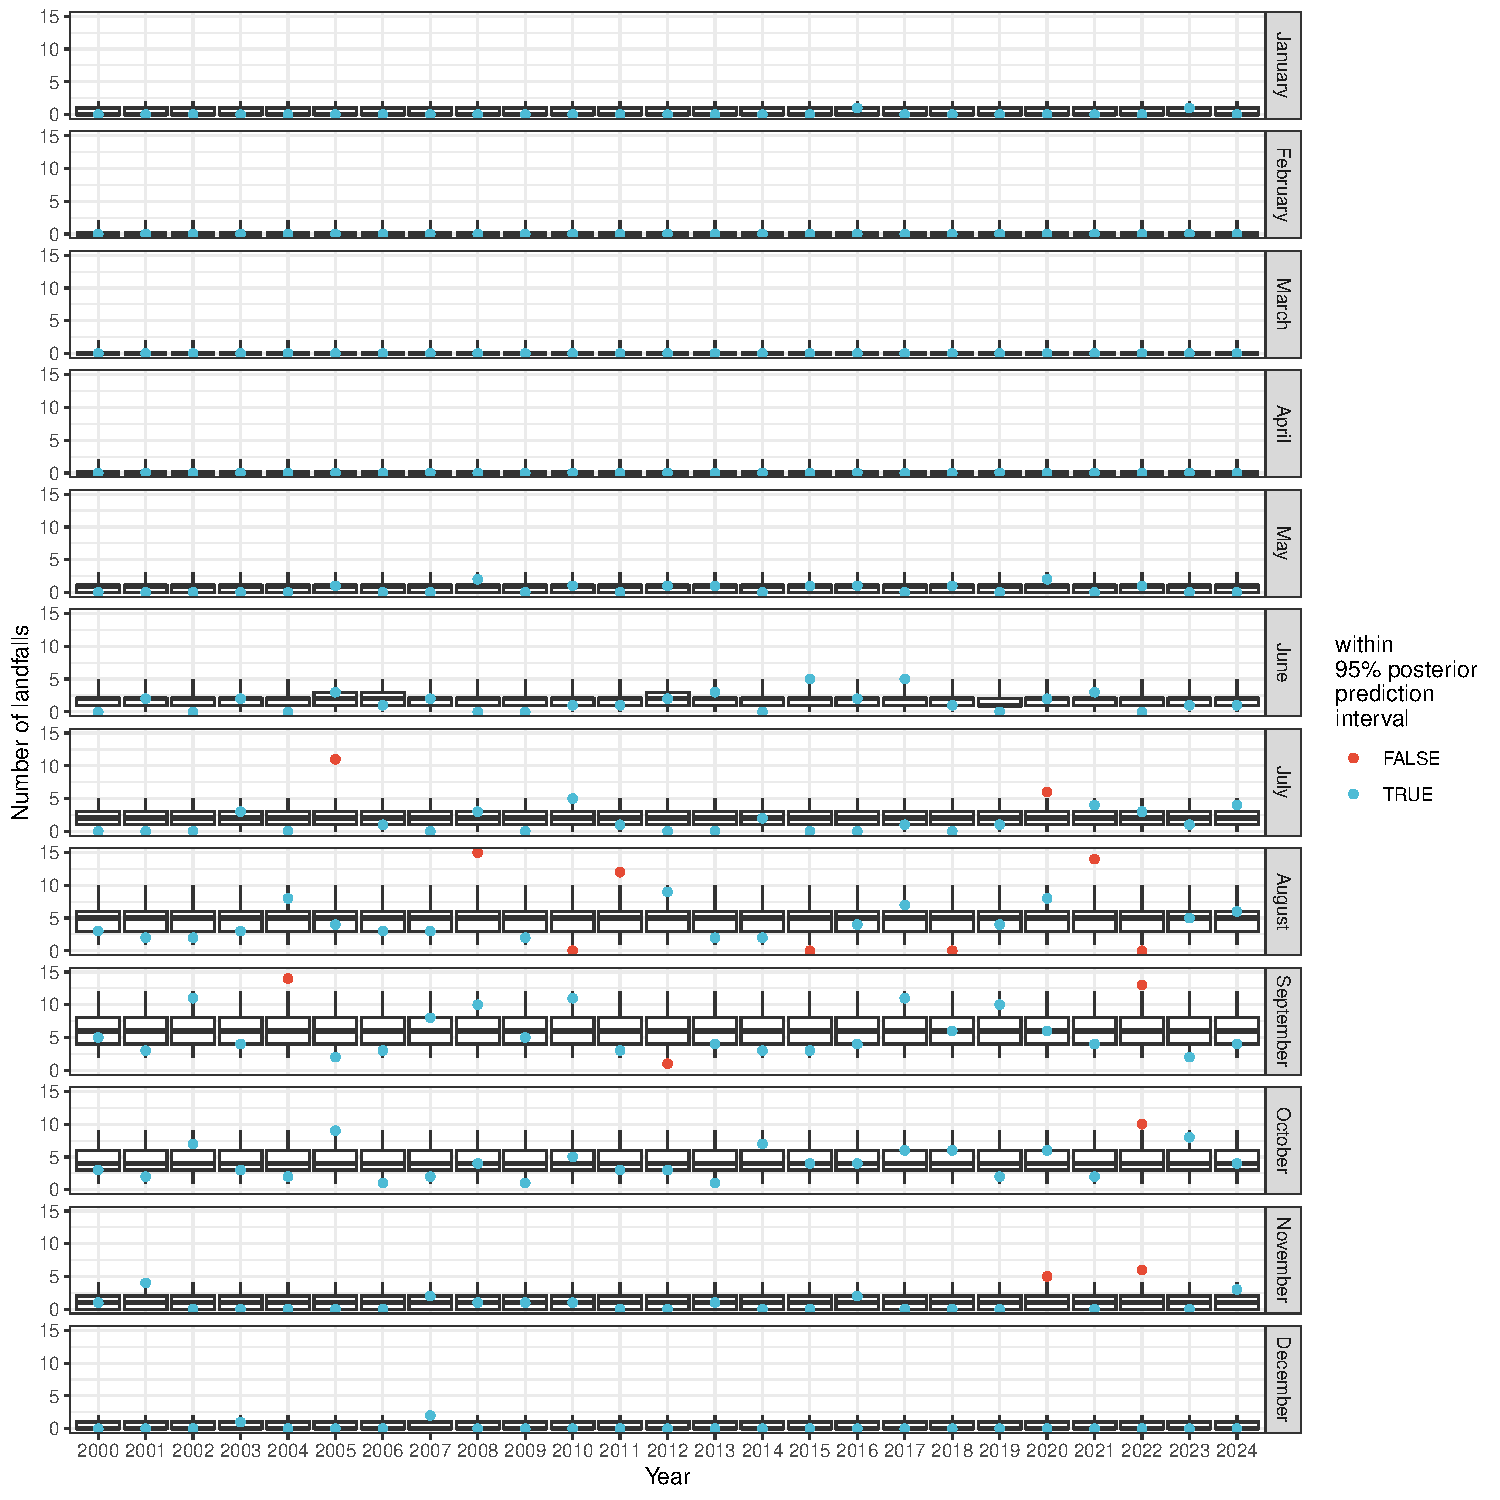
\includegraphics[width=1\linewidth]{../outputs/bayesian-analysis-landfall-freq/model-no-year-effect/no-year-post-pred-checks} 

}

\caption{95\% posterior credible intervals and observed data for each month and year, 2000-2024.}\label{fig:figs12}
\end{figure}

We found that 95\% of our observed landfall counts fell within our model's posterior predictive intervals, suggesting a good model fit. This can be seen in Figure \ref{fig:figs12}.

\newpage

\subsection{Model A and Model B Comparison}\label{model-a-and-model-b-comparison}

To compare the predictive performance of our models A and B, we computed the expected log posterior predictive density (ELPD) using approximate Leave-One-Out (LOO) Cross Validation. This is a statistic commonly used in Bayesian statistics to measure how well a model predicts unseen data, where the model with higher ELPD value is preferred.

\begin{figure}

{\centering 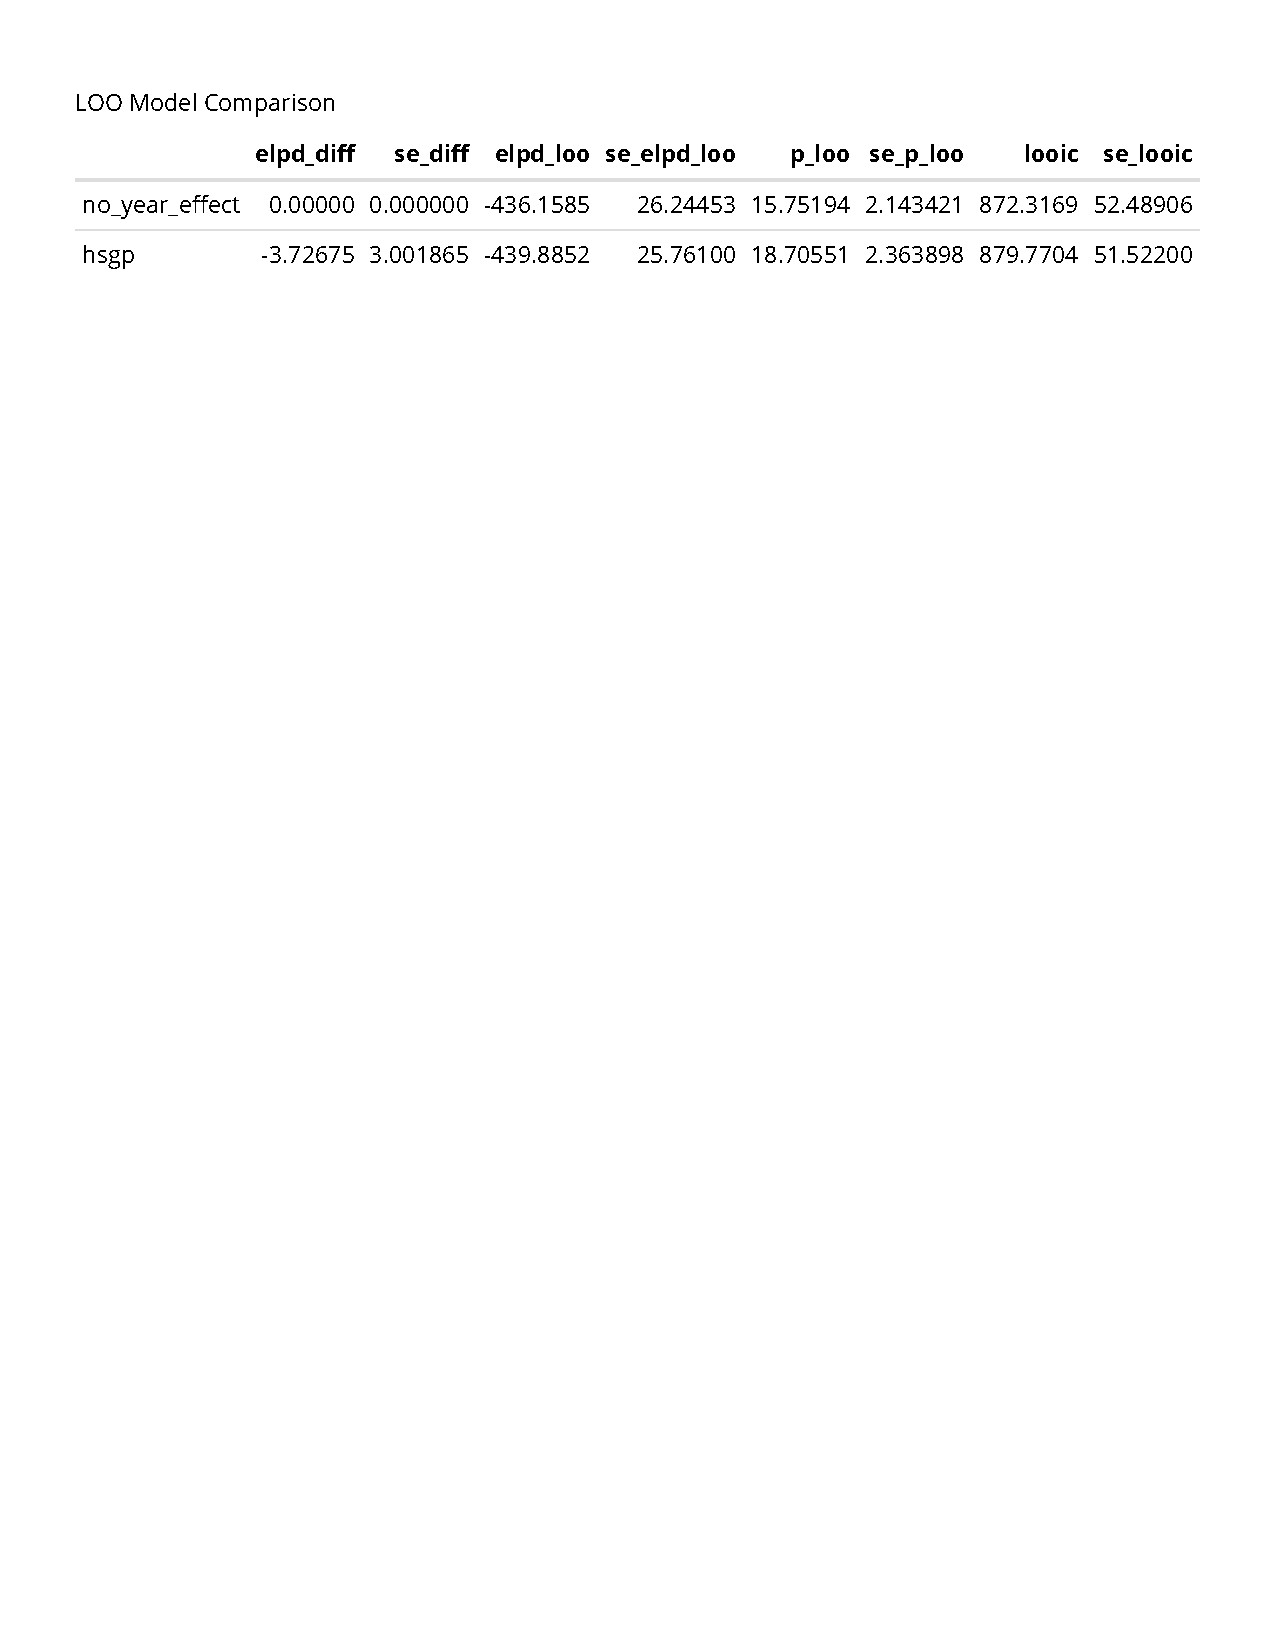
\includegraphics[width=1\linewidth]{../outputs/bayesian-analysis-landfall-freq/best-model-comp} 

}

\caption{LOO Cross Validation measures for comparative model performance.}\label{fig:figs13}
\end{figure}

Figure \ref{fig:figs13} shows model performance comparison measures such as:

\begin{itemize}
\tightlist
\item
  elpd\_diff: Difference in ELPD between models
\item
  se\_diff: Standard error of the difference in ELPD
\item
  elpd\_loo: ELPD value using LOO cross-validation
\item
  se\_elpd\_loo: Standard error of the ELPD for LOO cross-validation
\end{itemize}

The difference in ELPD between Model B and Model A is approximately 3.73, as can be seen in Figure \ref{fig:figs13}, with a standard error of 3.00. This suggests that Model B has a slightly better predictive performance, but overall, both models behave similarly as this difference is marginal. For simplicity, we used Model B to forecast landfalls per month and year.

\subsection{Model C: Geographical model}\label{model-c-geographical-model}

For our final geographical model, our Bayesian Poisson regression model now includes a location (country or territory) effect. This model was then fitted using Markov Chain Monte Carlo (MCMC) methods.

Mathematically, our model is denoted:

\begin{align*}
&Y_{i} \sim \text{Poisson}(\lambda_{i})\\
&\text{log } \lambda_{i} =  \beta_0 + X \beta\\
&\beta_0 \sim \text{Normal}(0,2^2)\\
&\sigma_{\beta} \sim \text{Half-Cauchy}(0,1)\\
&\beta \sim \text{MVN}( 0, \frac{L}{L-1}( I - \frac{1}{L} \mathbf{1}\mathbf{1}^T) \cdot \sigma_{\beta}^2), \text{ (sum-to-zero parameterisation)}\\
\end{align*}

where

\begin{itemize}
\tightlist
\item
  \(i\) indexes observations, \(i=1,...,250\);
\item
  \(j\) indexes the countries or territories, \(j = 1,...,10\);
\item
  \(L\) is the number of countries/territories, \(L=10\);
\item
  \(Y_{i}\) is the observed count of landfalls for observation \(i\);
\item
  \(X\) is a \(300 \times 10\) dimensional design matrix consisting of one-hot columns for each location;
\item
  \(\beta_0\) is the baseline parameter;
\item
  \(\beta \in \mathbb{R}^{10}\) is the monthly seasonal effect, where \(\beta_1\) is the effect for country/location 1, \(\beta_2\) is the effect for country/territory 2 and so on;
\item
  \(\sigma_{\beta}\) scales the variance of \(\beta\) to implement non-centered parameterisation on top of the sum-to-zero constraint, where both constraints were implemented to improve parameter identifiability, sampling efficiency and convergence of our model parameters;
\item
  \(\lambda_{i}\) is the expected number of landfalls per month and year
\end{itemize}

We ran our MCMC algorithm using 3 parallel Markov chains, 6000 iterations, discarding the first 500 as ``warm-up'' iterations. We verified model convergence by investigating key model parameter convergence diagnostics, as well as checking the trace plot for our worst performing parameter and looking at pairwise posterior geometries.

\begin{figure}

{\centering 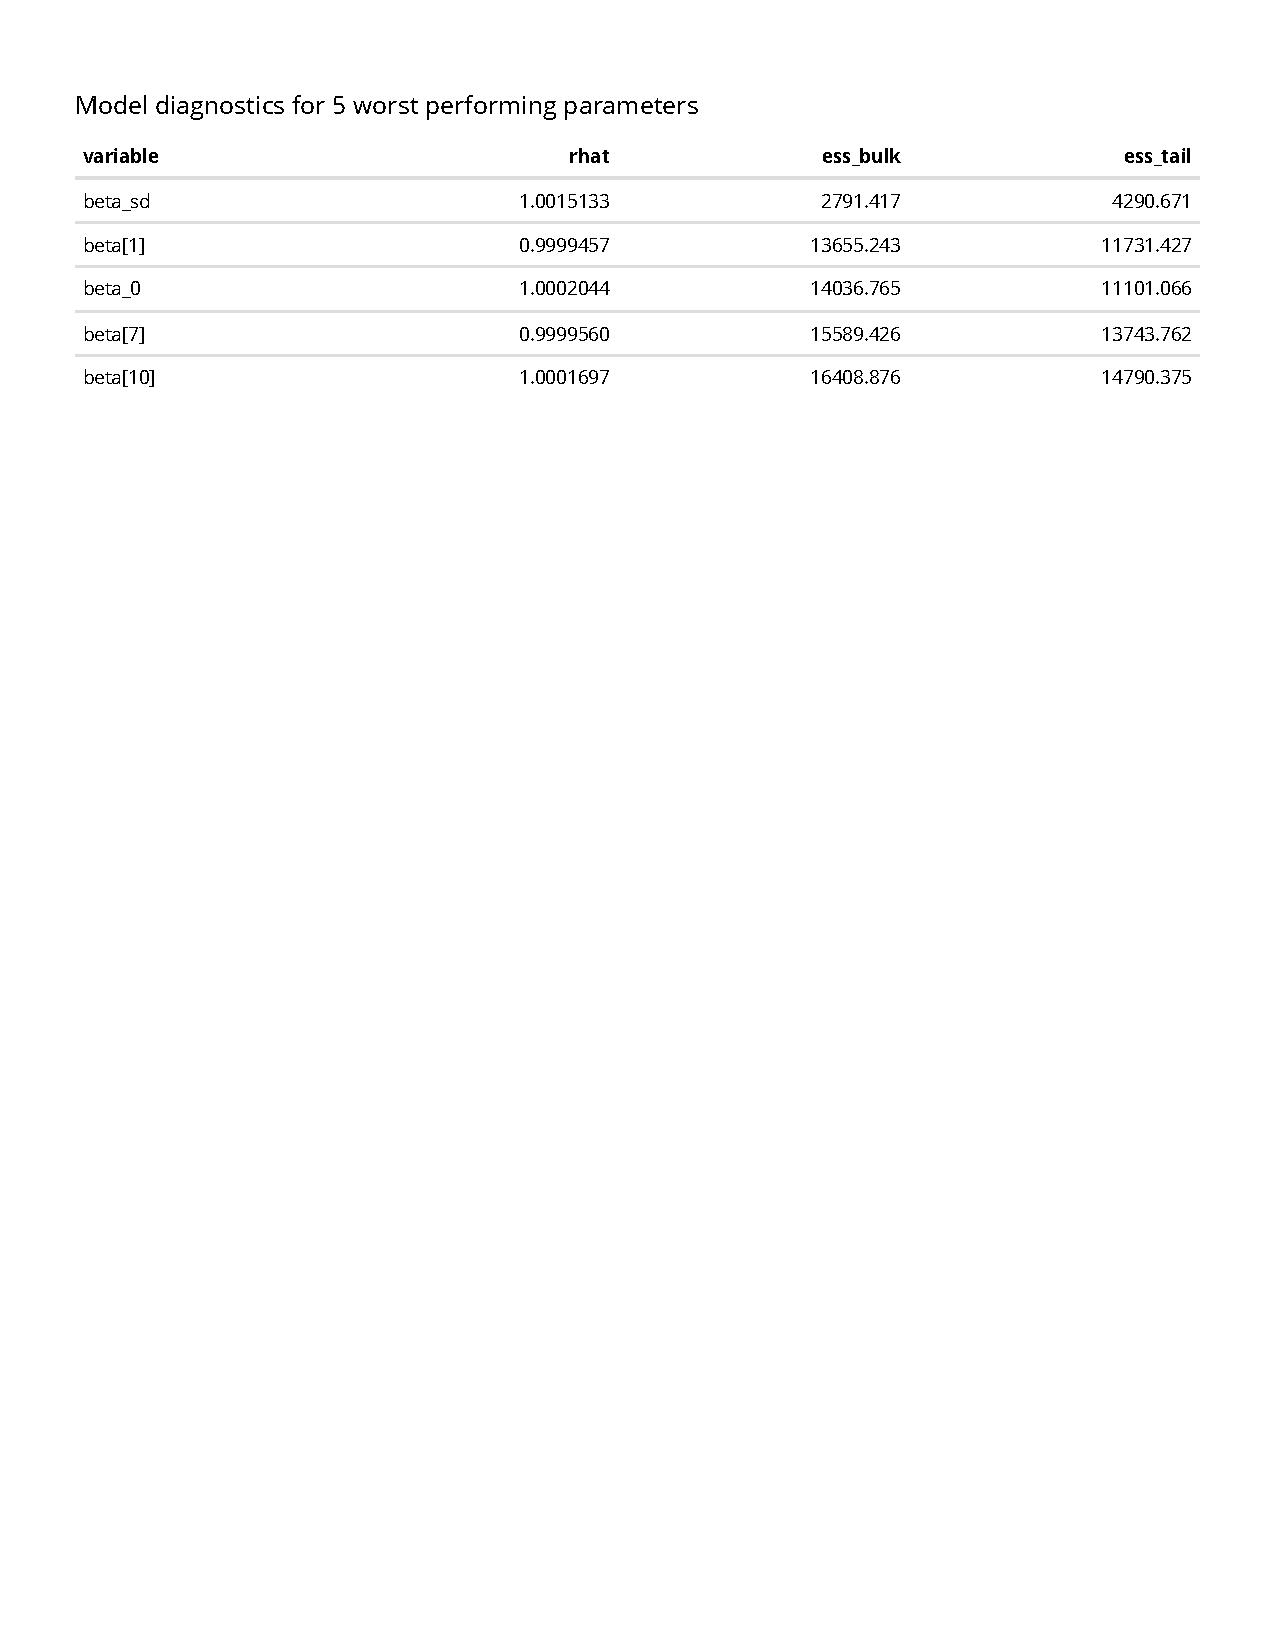
\includegraphics[width=1\linewidth]{../outputs/bayesian-analysis-country-freq/country-model-diagnostics} 

}

\caption{Model convergence diagnostics for our 5 worst performing parameters.}\label{fig:figs14}
\end{figure}

Figure \ref{fig:figs14} displays the 3 statistical efficiency and convergence measures for our worst performing parameters (in terms of the ``ess\_bulk'' measure). As we can see, all ``rhat'' convergence diagnostic values are less than 1.01, which suggests good mixing and convergence. Moreover both ``ess\_tail'' and ``ess\_bulk'' are above 1500, suggesting good sampling efficiency.

We then checked model fit by performing a posterior predictive check, similarly to Models A and B.

\begin{figure}

{\centering 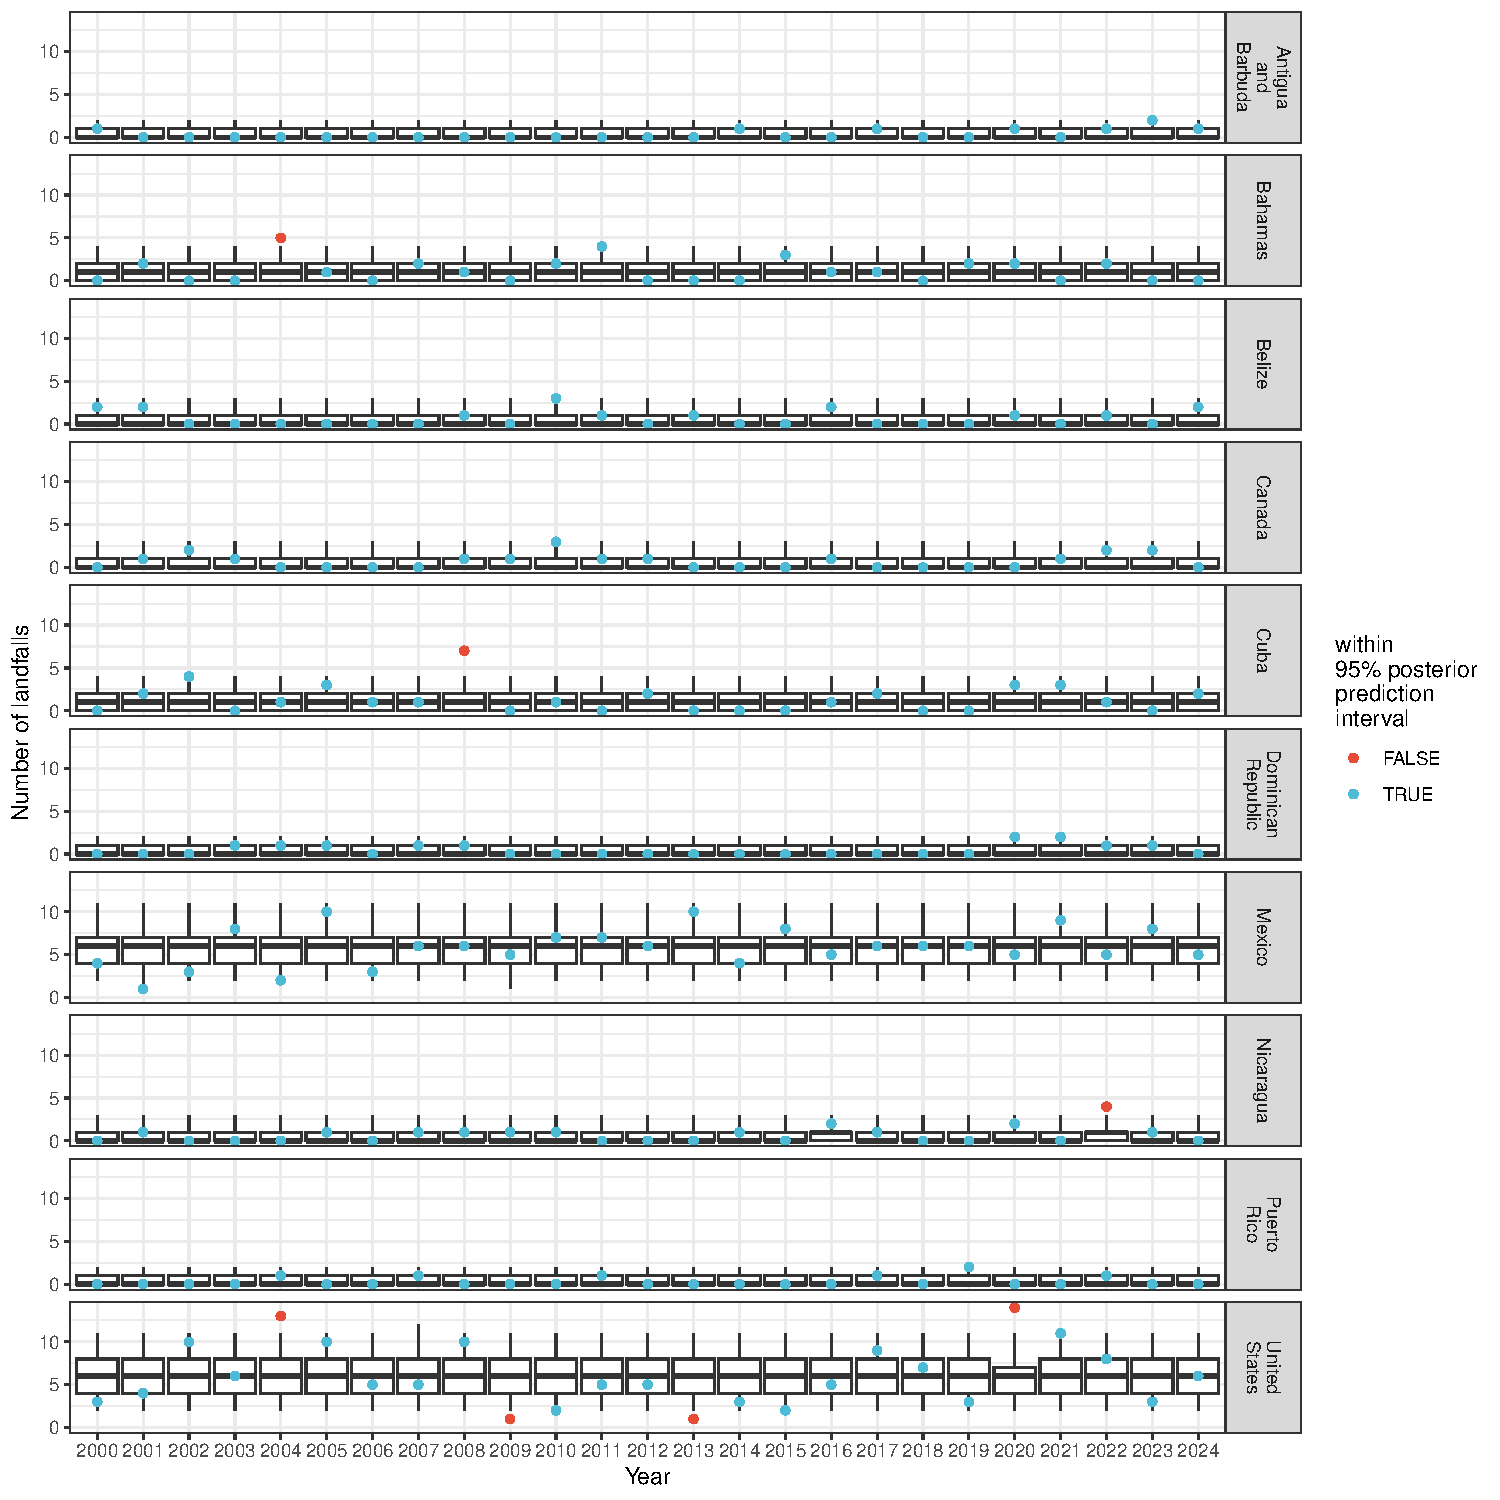
\includegraphics[width=1\linewidth]{../outputs/bayesian-analysis-country-freq/country-post-pred-checks} 

}

\caption{95\% posterior credible intervals and observed data for each month and year, 2000-2024.}\label{fig:figs15}
\end{figure}

We found that 96.8\% of our observed landfall counts fell within our model's posterior predictive intervals, suggesting a good model fit. This can be seen in Figure \ref{fig:figs15}.

\end{document}
